\documentclass{article}
\usepackage[margin=2.5cm, includefoot, footskip=30pt]{geometry}

\setlength{\parindent}{0em}
\setlength{\parskip}{1em}
\renewcommand{\baselinestretch}{1}

%%%%Packages%%%%
\usepackage{amsmath}
\usepackage{booktabs}
\usepackage{graphics}
\usepackage{multicol}
\usepackage[ruled,vlined]{algorithm2e}
\usepackage{setspace}
\usepackage{graphicx}
\usepackage{subcaption}
\usepackage{hyperref}
\usepackage{color,colortbl}
\usepackage{array}
\usepackage{booktabs}
\usepackage{tabularx}
\usepackage{wrapfig, blindtext}
%%%%%%%%%%%%%%%%%

\definecolor{Gray}{gray}{0.92}
\usepackage[first=0,last=9]{lcg}
\newcommand{\ra}{\rand0.\arabic{rand}}

\setlength{\tabcolsep}{3pt}

\title{A meta analysis of tournaments and an evaluation of performance in the
Iterated Prisoner's Dilemma.}
\author{Nikoleta E. Glynatsi, Dr Vincent A. Knight}
\date{}

\begin{document}

\maketitle

\begin{abstract}

The Iterated Prisoner's Dilemma has been used for decades as a powerful model of
behavioural interactions. From the celebrated performance of Tit for Tat, to the
introduction of the zero-determinant strategies, to the use of sophisticated
structures such as neural networks, the literature has been exploring the
performance of strategies in the game for years. Most of these strategies are
now accessible due to an open source package; Axelrod-Python. This manuscript
make use of Axelrod-Python to conduct a meta analysis of 40000 Iterated
Prisoner's Dilemma tournaments. The aim is to evaluate the performance of
numerous strategies and finally answer the explore the factors of success in the
game.
\end{abstract}

\section{Background}

The Iterated Prisoner's Dilemma (IPD) is a repeated two player game that models
situations in which self-interest clashes with collective interest. At each turn,
the players simultaneously and independently make a choice between cooperation (C) and
defection (D) whilst having memory of the prior interactions.
The payoffs at each given turn are defined by the matrix,

\[\begin{pmatrix}
R & S \\
T & P
\end{pmatrix}\]

where \(T > R > P > S\) and \(2R > T + S\). The most common values used in
the literature, and in this paper, are $R=3, P=1, T=5, S=0$.

Since the computer tournaments of R. Axelrod in 1980s several academic papers
are published in the field regarding the performance of strategies in the
IPD. In the 80's following the strong performance of Tit For Tat
in both Axelrod's computer tournaments~\cite{Axelrod1980a, Axelrod1980b}, and
moreover in a series of evolutionary experiments~\cite{Axelrod1981}, the strategy
was thought as the most robust basic strategy in the iterated prisoner's
dilemma. However, the strategy's poor performance in environments with
noise~\cite{Bendor1991, Donninger1986, Molander1985, Hammerstein1984},
made room for other protagonists, such as, Nice and Forgiving~\cite{Bendor1991},
Pavlov~\cite{Nowak1993} and Generous Tit For Tat~\cite{Nowak1992}.

In 2004, the Anniversary Iterated Prisoner Dilemma Tournament was run with 233
entries. The winning strategies were based on a mechanism of teams. A team from
Southampton University took advantage of the fact that a participant was allowed
to submit multiple strategies. They submitted a total of 60 of strategies that
could recognised each other and colluded to increase one members
score~\cite{J.P.Delahaye1993Lp, J.P.Delahaye1995LIeP, A.Rogers2007Ctpw}.

Yet again, in 2012 another set of strategies was introduced as the dominant set
of strategies~\cite{Press2012}. These were called zero-determinant strategies,
and by forcing a linear relationship between the payoffs they can ensure that
they will never receive less than their opponents. However, in~\cite{Harper2017}
a tournament containing over 200 strategies, zero-determinant, was performed and
none of the zero-determinant strategies ranked in top spots. Instead, the top
ranked strategies were a set of evolved strategies based lookup tables, hidden
markov models and finite state automata.
%TODO reference the archetypes of the archetypes used the IPD?

Thus, the following question is raised here: which are the true dominant
strategies in the iterated prisoner's dilemma?
This manuscript uses the open source package
Axelrod-Python~\cite{axelrodproject} to simulate a large number of computer
tournaments using as many strategies as possible from the literature. The aim is
to evaluate the performance of these strategies in a tournament and futhermore,
explore the factors of their success. This is done not for standard round robin
tournaments, but also for noisy, probabilistic ending and noisy probabilistic
ending tournaments.

The different tournaments and the data generating process are covered in
Section~\ref{section:data_collection}. Section~\ref{section:top_performances},
covers the best performed strategies for each type of tournament and overall.
Section~\ref{section:evaluation_of_performance}, explores the traits which
contribute to good performance and finally in Section~\ref{section:conclusion}
the results are discussed and summarised.

\section{Data generating process}\label{section:data_collection}

For the purposes of this manuscript a data set containing results on IPD tournaments
has been generated and is available at. This
was done using the open source package Axelrod-Python~\cite{axelrodproject},
more specifically, version 3.0.0. Axelrod-Python allows for different types of
IPD computer tournaments to be simulated whilst
containing a list of over 180 strategies. Most of these are strategies described
in the literature with a few exceptions being strategies that have been
contributed specifically to the package. Though Axelrod-Python features several
tournament types, this work considers only standard, noisy, probabilistic ending
and noisy probabilistic ending tournaments.

\textbf{Standard tournaments}, are tournaments similar to that of Axelrod's
in~\cite{Axelrod1980a}. There are \(N\) strategies which all play an iterated
game of \(n\) number of turns against each other. Note that self interactions
and a match against a random strategy are not included. Similarly, \textbf{noisy
tournaments} have \(N\) strategies and \(n\) number of turns but at each turn
there is a probability \(p\) that a player's action will be flipped.
\textbf{Probabilistic ending tournaments}, are of size \(N\) and after each turn
a match between strategies ends with a given probability \(e\). Finally,
\textbf{noisy probabilistic ending} tournaments have both a noise probability
\(p\) and an ending probability \(e\). For smoothing the simulated results a
tournament is repeated for \(k\) number of times. The winner of each tournament
is based on the average score a strategy achieved and not by number of wins.

%  A summary of
% each tournaments' parameters is given in Table~\ref{table:tournaments_parameters}.

% \begin{table}[!htbp]
%     \begin{center}
%         \resizebox{.85\textwidth}{!}{
%         \begin{tabular}{lcccccc}
%     \toprule
%     tournament type & number of strategies & repetitions & turns & noise probability & probability of match ending \\
%     \midrule
%     standard & $N$ & k & $n$ & - & - \\
%     noisy & $N$  & k & $n$ & $p$ & - \\
%     probabilistic ending & $N$ & k & - & - & $e$ \\
%     noisy probabilistic ending & $N$ & k & - & $p$ & $e$ \\
%     \bottomrule
%         \end{tabular}}
%     \end{center}
%     \caption{Tournament types' parameters.}
%     \label{table:tournaments_parameters}
% \end{table}

The process of generating data implemented in this manuscript is given by
Algorithm~\ref{algorithm:data_generation}. For each trial a random
size \(N\) is selected, and from the list of 186 strategies
in~\cite{axelrodproject}, a random list of \(N\) strategies is chosen. For the
given list of strategies a standard, a noisy, a probabilistic ending and a noisy
probabilistic ending tournament are performed and repeated \(k\) times.
The parameters for the tournaments as well as the number of repetitions are
selected once for each trial. The parameters and their respective minimum and
maximum values are given by Table~\ref{table:parameters_values}.

\begin{table}[!htbp]
    \begin{center}
        \resizebox{.6\textwidth}{!}{
        \begin{tabular}{lcccc}
    \toprule
    parameter & parameter explanation &   min value & max value \\
    \midrule
    $N$ & number of strategies  & 3 & 195 \\
    $k$ & number of repetitions  & 10 & 100 \\
    $n$ & number of turns      & 1 & 200 \\
    $p$ & probability of flipping action at each turn  & 0 & 1   \\
    $e$ & probability of match ending in the next turn & 0 & 1   \\
    \bottomrule
        \end{tabular}}
    \end{center}
    \caption{Data generation parameters' values}
    \label{table:parameters_values}
\end{table}

The source code for the data generating process as well as the source code for
the analysis which will be discussed in the following sections have been written
following best practices~\cite{Aberdour2007, Benureau2018}. It has been packaged
and is available here.

\begin{algorithm}[!htbp]
    \setstretch{1.35}
    \ForEach{\text{seed} $\in [0, 12285]$}{
        $N \gets \text{randomly select integer}\in [N_{min}, N_{max}]$\;
        $\text{players} \gets  \text{randomly select $N$ players}$\;
        $k \gets  \text{randomly select integer}\in [k_{min}, k_{max}]$\;
        $n \gets  \text{randomly select integer}\in [n_{min}, n_{max}]$\;
        $p \gets  \text{randomly select float}\in [p_{min}, p_{max}]$\;
        $e \gets   \text{randomly select float}\in [e_{min}, e_{max}]$\;
        \vspace{0.4cm}
        $\text{result standard}$ $\gets$ Axelrod.tournament$(\text{players}, n, k)$\;
        $\text{result noisy}$ $\gets$ Axelrod.tournament$(\text{players}, n, p, k)$\;
        $\text{result probabilistic ending}$ $\gets$ Axelrod.tournament$(\text{players}, e, k)$\;
        $\text{result noisy probabilistic ending}$ $\gets$ Axelrod.tournament$(\text{players}, p, e, k)$\;

    }
    \KwRet{result standard, result noisy, result probabilistic ending,
    result noisy probabilistic ending}\;
    \caption{Data generating Algorithm}
    \label{algorithm:data_generation}
\end{algorithm}

A total of 12,285 trials of Algorithm~\ref{algorithm:data_generation} have been
performed. For each trial the results for 4 different tournaments were collected,
thus a total of 49,140 $(12,285 \times 4)$ tournament results have been
retrieved. Each tournament outputs a result summary in the form of
Table~\ref{table:output_result}.

The result summary has a length \(N\) because each row contains information for
each strategy that participated in the tournament. The information include the
strategy's rank, median score, the rate with which the strategy cooperated
$(C_r)$, it's wins and the probability that the strategy cooperated in the
opening move. Moreover, the rates of a strategy being in any of the four states
($CC, CD, DC, DD$), and the rate of which the strategy cooperated after each
state.

\newcolumntype{g}{>{\columncolor{Gray}}c}
\begin{table}[!htbp]
    \begin{center}
    \resizebox{\textwidth}{!}{
    \begin{tabular}{ccccccgcgcgcgcg}
    \toprule 
    & & & & & &   \multicolumn{8}{g}{Rates}  \\
    Rank & Name & Median score & Cooperation rating $(C_r)$ & Win & Initial C &
    CC & CD & DC & DD & CC to C & CD to C & DC to C & DD to C \\
    0 &  EvolvedLookerUp2 2 2 & 2.97 & 0.705 & 28.0 & 1.0 & 0.639 & 0.066 & 0.189 &
    0.106 & 0.836 & 0.481 & 0.568 & 0.8 \\
    1 &  Evolved FSM 16 Noise 05 & 2.875 & 0.697 & 21.0 & 1.0 & 0.676 & 
    0.020 & 0.135 & 0.168 & 0.985 & 0.571 & 0.392 & 0.07 \\
    2 & PSO Gambler 1 1 1 & 2.874 & 0.684 &  23.0 &     1.0 &    0.651 &    0.034 &    0.152 &    0.164
    & 1.000 & 0.283 & 0.000 & 0.136 \\
    3 &  PSO Gambler Mem1 &  2.861 &        0.706 &  23.0 &      1.0 &    0.663
    &    0.042 &    0.145 &    0.150 &  1.000 &  0.510 &  0.000 &  0.122 \\
    4 &          Winner12 &  2.835 &        0.682 &  20.0 &      1.0 &
    0.651 &    0.031 &    0.141 &    0.177 &  1.000 &  0.441 &  0.000 &  0.462 \\
    $\dots$ & $\dots$ & $\dots$ & $\dots$ & $\dots$ & $\dots$ & $\dots$ & $\dots$ &
    $\dots$ & $\dots$ & $\dots$ & $\dots$ & $\dots$ & $\dots$ \\
    \bottomrule
    \end{tabular}}
\end{center}
\caption{Output result.}\label{table:output_result}
\end{table}

The normalised rank is a measure which was manually included. The normalised
rank, denoted as $r$, is calculated as a strategy's rank divided by the
tournament's size ($N$). The normalised rank will be used in the next section to
evaluate the performance of strategies.

\section{Top ranked strategies}\label{section:top_performances}

This section evaluates the performance of 186 strategies which can be found in
the Appendix. The performance of each strategy will be evaluated for each type
of tournament independently. In Section~\ref{subsection:standard_tournament} the
strategies are evaluated on their performance in standard tournaments, in
Section~\ref{subsection:noisy_tournament} in noisy, in
Sections~\ref{subsection:probend_tournament} in probabilistic ending and in
\ref{subsection:noisy_probend_tournament} in noisy probabilistic ending.

Each strategy could have participated in multiple tournaments of the same type
(on average each participated in 5690 different tournaments). For example Tit
For Tat has participated in a total of 5569 standard tournaments. The strategy's
normalised rank distribution in different tournament is given in
Figure~\ref{fig:tit_for_tat_r_distribution}. As a result, of the multiple
entries of strategies their performance is evaluated based on the median
normalised rank denoted as \(\bar{r}\). A value of \(\bar{r} = 0\) corresponds
to a strategy winning the tournament where a a value of \(\bar{r} = 1\)
corresponds to the strategy coming last.

\begin{figure}[!htbp]
    \centering
    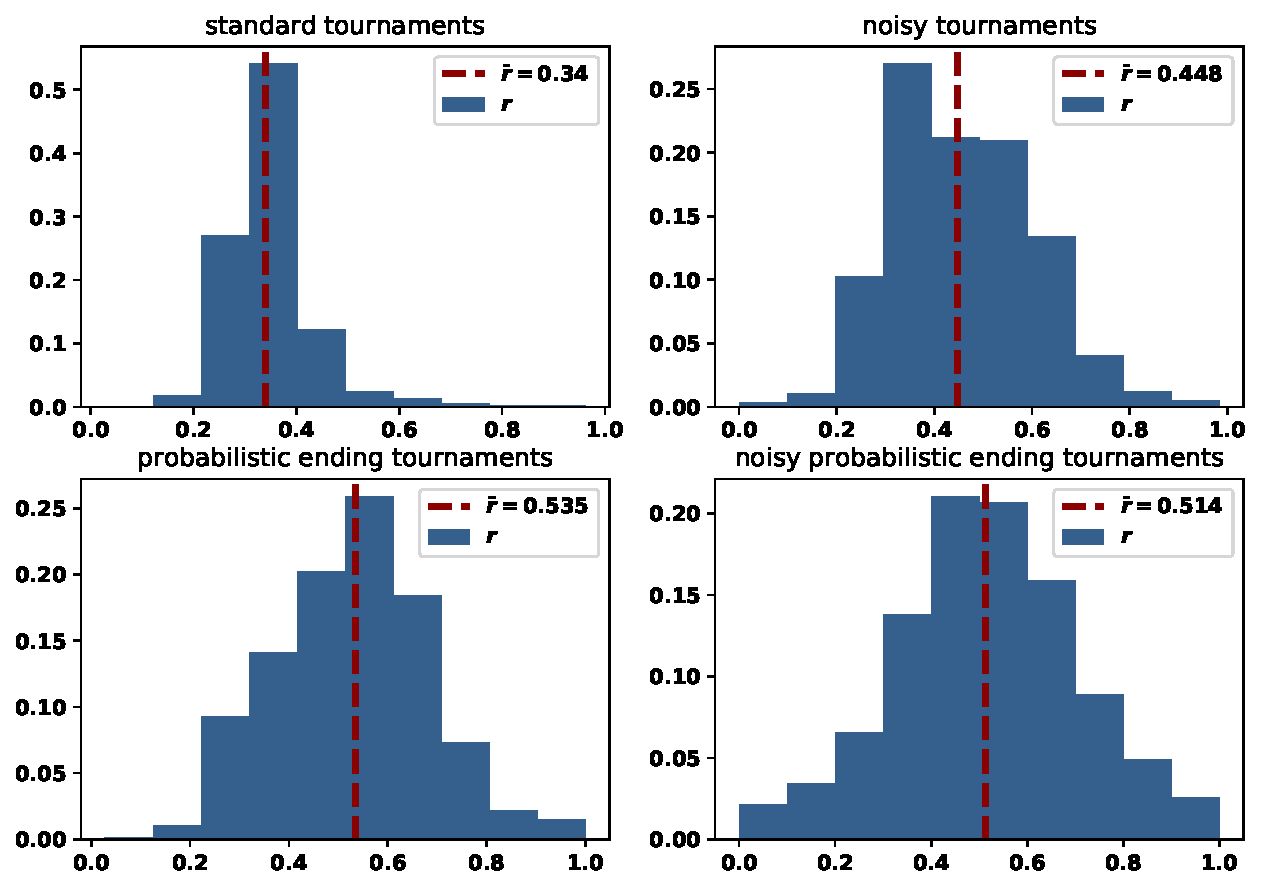
\includegraphics[width=.8\textwidth]{../images/tit_for_tat_r_distributions.pdf}
    \caption{Tit For Tat's $r$ distribution in tournaments.}
    \label{fig:tit_for_tat_r_distribution}
\end{figure}

Following the analysis of each tournament type, in Section~\ref{subsrction:overall}
the results are merged and the strategies are evaluated in their overall performances
over all simulated tournaments of this work.

\subsection{Top ranked strategies in: Standard tournaments}\label{subsection:standard_tournament}

The results presented in this section are based on $12,285$ different standard
tournaments.
The top 15 performances in standard tournaments are given in
Table~\ref{table:std_results}. Ten of these are strategies introduced
in~\cite{Harper2017}. These have been trained using reinforcement learning
algorithms and are based on finite state automata (FSM), hidden markov models
(HMM), artificial neural networks (ANN), lookup tables (LookerUp) and stochastic
lookup tables (Gambler). Specifically, the have been trained against the
strategy list of~\cite{axelrodproject} in standard tournaments. Thus their
performance is to be expected. DoubleCrosser, and Fool Me Once, are not from
the literature but from~\cite{axelrodproject}. DoubleCrosser is a strategy that
makes use of the length of the match because is set to defect on the last two
rounds. The strategy is expected to not perform as well in probabilistic ending
tournaments. Finally, Winner 12~\cite{Mathieu2017} and DBS are both from the the
literature. DBS~\cite{Au2006} is strategy specifically designed for noisy
environments, however, it ranks highly only in standard ones.

\begin{table}[!htbp]
    \centering
    \resizebox{.28\textwidth}{!}{
    \begin{tabular}{lr}
\toprule
{} &  $\bar{R}$ in standard tournaments \\
Name                    &                                    \\
\midrule
Evolved HMM 5           &                           0.006579 \\
Evolved FSM 16          &                           0.009901 \\
EvolvedLookerUp2\_2\_2    &                           0.010638 \\
Evolved FSM 16 Noise 05 &                           0.016393 \\
PSO Gambler 2\_2\_2       &                           0.021390 \\
Evolved ANN             &                           0.028736 \\
Evolved ANN 5           &                           0.033898 \\
PSO Gambler 1\_1\_1       &                           0.037234 \\
Evolved FSM 4           &                           0.048387 \\
PSO Gambler Mem1        &                           0.050000 \\
Winner12                &                           0.059459 \\
Fool Me Once            &                           0.061224 \\
DBS                     &                           0.070866 \\
DoubleCrosser           &                           0.071895 \\
BackStabber             &                           0.075000 \\
\bottomrule
\end{tabular}
}
    \caption{Standard top performances}\label{table:std_results}
\end{table}

Figure~\ref{fig:std_results} gives the distributions of $\bar{r}$ for the top
ranked strategies. The distributions are skewed towards zero and the highest
median is at 0.075. This indicates that the top ranked strategies are dominating
strategies in standard tournaments. They are very likely to perform well in
standard tournament despite the number of opponents, the opponents, the turns
etc. This does not hold for all the tournament types as it will be discussed
in the following sections. The next section present the results of noisy
tournaments.

\begin{figure}[!htbp]
    \centering
    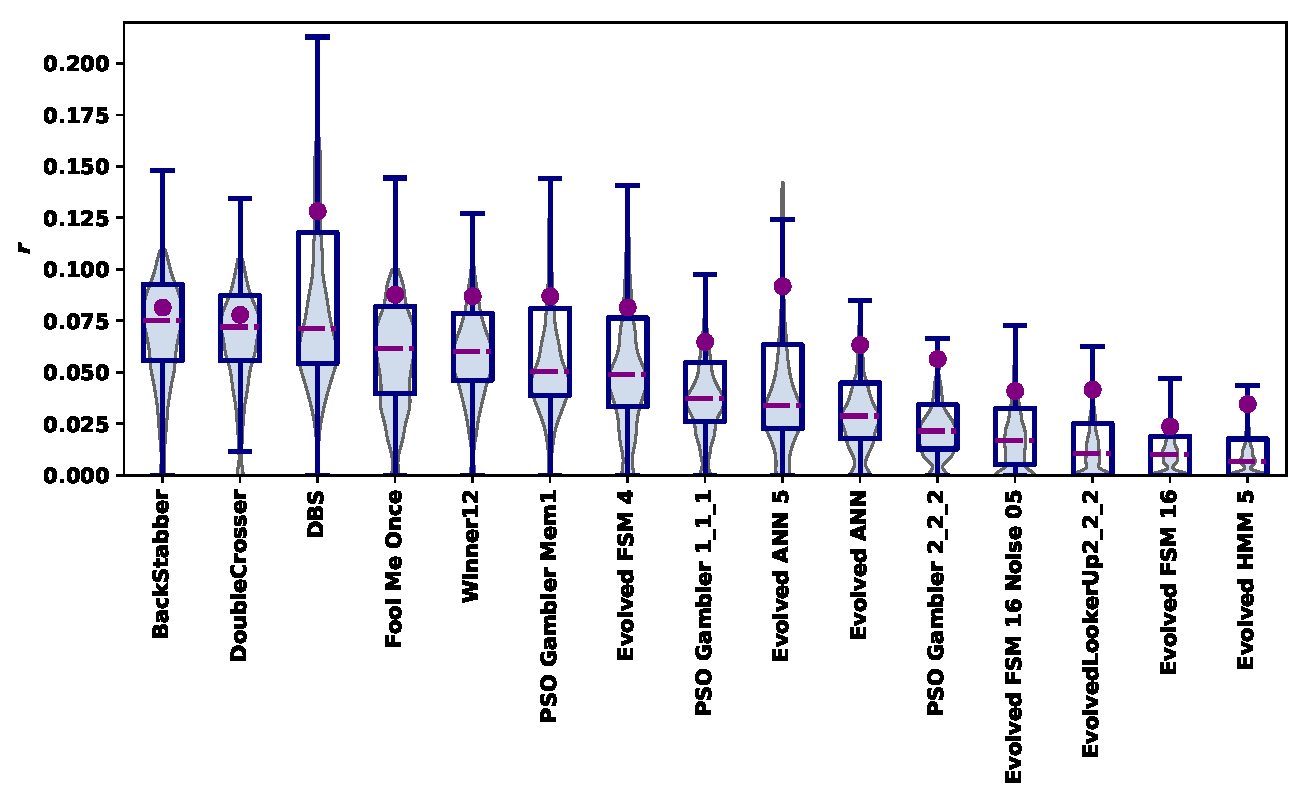
\includegraphics[width=.7\textwidth]{../images/performance_standard.pdf}
    \caption{$\bar{r}$ distributions of top 15 strategies.}\label{fig:std_results}
\end{figure}

\subsection{Top ranked strategies in: Noisy tournaments}\label{subsection:noisy_tournament}

Similarly to Section~\ref{subsection:standard_tournament} the results presented
here are based on $12,285$ different noisy tournaments. The strategies have been
ranked based on their \(\bar{r}\) and the top 15 are given by
Table~\ref{table:noisy_results}. The distributions of their corresponding
\(\bar{r}\) is also given in Figure~\ref{fig:noisy_results}.

The top strategies include the two strategies, Tit For 2
Tats~\cite{Axelrod1980b} and Hard Tit For 2 Tats~\cite{Stewart2012}, which are
strategies that will defect only after the have received two defections from the
opponent. The Retaliate strategies are set of strategies
from~\cite{axelrodproject} that start by cooperating but will retaliate once the
opponent's wins and defections surpass a curtain threshold.
ShortMem~\cite{Carvalho2013}, Grumpy, $e$ and $\phi$ are strategies that make
decisions based on the cooperations to defections ratio. In $5^{\text{th}}$ and
$6^{\text{th}}$ place are the strategies Cycler Hunter and  Risky QLearn. Cycler
Hunter tries to extort strategies that play cyclically and Risky QLearn uses a Q
learning algorithm. Notably, a deterministic and one of the most simple
strategies in game is ranked $3^{\text{rd}}$. That is Cooperator, a strategy
that just cooperates.

\begin{table}[!htbp]
    \centering
    \resizebox{.25\textwidth}{!}{
    \begin{tabular}{lr}
\toprule
Name                &                        $\bar{r}$\\
\midrule
Grumpy              &                         0.13953 \\
$e$                 &                         0.19048 \\
Cooperator          &                         0.19565 \\
Tit For 2 Tats      &                         0.20520 \\
Cycle Hunter        &                         0.22222 \\
Risky QLearner      &                         0.22424 \\
Retaliate 3         &                         0.23077 \\
Retaliate 2         &                         0.23762 \\
Retaliate           &                         0.24309 \\
Hard Tit For 2 Tats &                         0.24658 \\
Limited Retaliate 3 &                         0.25000 \\
ShortMem            &                         0.25272 \\
Limited Retaliate   &                         0.25698 \\
Limited Retaliate 2 &                         0.26027 \\
$\phi $              &                         0.26201 \\
\bottomrule
\end{tabular}
}
    \caption{Noisy top performances}\label{table:noisy_results}
\end{table}

From Figure~\ref{fig:std_results} it is evident that the normalised rank distributions
in noisy environments are more variant and have higher median values compared
to standard tournaments. The distributions are skewed both towards
0 and 1 which indicates that though the top ranked strategies mainly
performed well (medians $< 0.3$) there are several tournaments that they performed
worse than the 60\% of the participants.

\begin{figure}[!htbp]
    \centering
    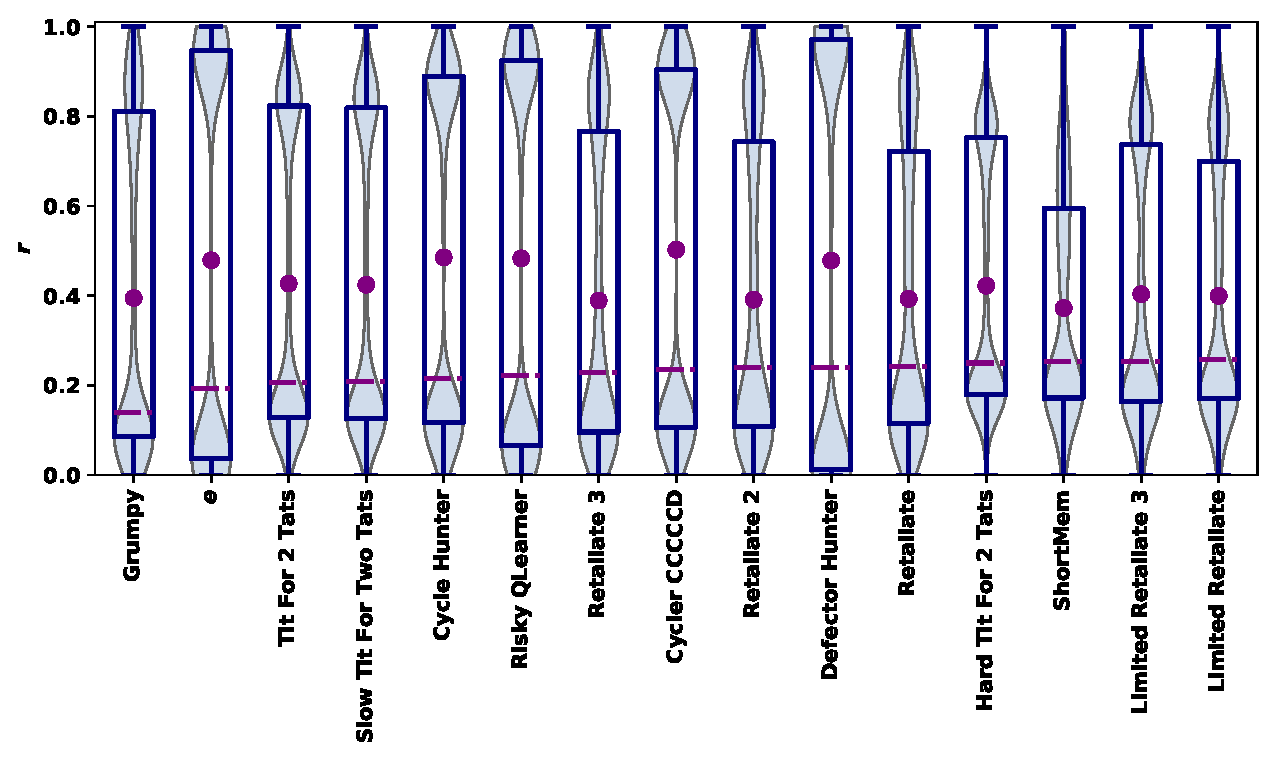
\includegraphics[width=.7\textwidth]{../images/performance_noise.pdf}
    \caption{\(\bar{r}\) distributions for best performed strategies in noisy tournaments.}
    \label{fig:noisy_results}
\end{figure}

\subsection{Top ranked strategies: Probabilistic ending tournaments}\label{subsection:probend_tournament}

In this section the performances in probabilistic ending tournaments are
discussed. The 15 top ranked strategies are given by
Table~\ref{table:prob_end_results} and Figure~\ref{fig:probend_results} gives
their respective $\bar{r}$ distributions.
Fortress 3, Fortress 4 (both introduced in~\cite{Ashlock2006}),
Raider~\cite{Ashlock2014} and Solution B1~\cite{Ashlock2014} are strategies
based on finite state automata introduced by Daniel and Wendy Ashlock. These
strategies have been evolved using reinformed learning, however, there were
trained to maximise their payoffs in tournaments with fixed turns (150
specifically) and not in probabilistic ending ones.

In probabilistic ending tournaments it appears that the top ranks are mostly
occupied by defecting strategies which include Better and Better, Gradual
Killer, Hard Prober (all from ~\cite{prison}), Bully (Reverse Tit For
Tat)~\cite{Nachbar1992} and Defector. Thus, it's surprisingly that EasyGo and
Fool Me Forever are ranked $14^{\text{th}}$ and $15^{\text{th}}$. These
strategies are actually the same; they will defect until their opponent defect,
then they will cooperate until the end. Both strategies have repeatedly ranked highly
as shown in Figure~\ref{fig:probend_results} and there are cases for which they
were the winners of tournaments.

\begin{table}[!htbp]
    \centering
    \resizebox{.25\textwidth}{!}{
    \begin{tabular}{lr}
\toprule
Name              &        $\bar{r}$                 \\
\midrule
Fortress4         &                           0.01266 \\
Defector          &                           0.01444 \\
Better and Better &                           0.01587 \\
Tricky Defector   &                           0.01869 \\
Fortress3         &                           0.02198 \\
Gradual Killer    &                           0.02521 \\
Aggravater        &                           0.02797 \\
Raider            &                           0.03077 \\
Cycler DDC        &                           0.04545 \\
Hard Prober       &                           0.05085 \\
SolutionB1        &                           0.06040 \\
Meta Minority     &                           0.06040 \\
Bully             &                           0.06061 \\
Fool Me Forever   &                           0.07018 \\
EasyGo            &                           0.07065 \\
\bottomrule
\end{tabular}
}
    \caption{Probabilistic ending top performances}\label{table:prob_end_results}
\end{table}

The distributions of the normalised rank in probabilistic ending tournaments are
less variant than those of noisy tournaments. The medians are lower than 0.1 and the
distributions are skewed towards 0. Though the large difference between the means
and the medians indicates some outliers, the strategies have overall performed
well in the tournaments that they participated.

\begin{figure}[!htbp]
    \centering
    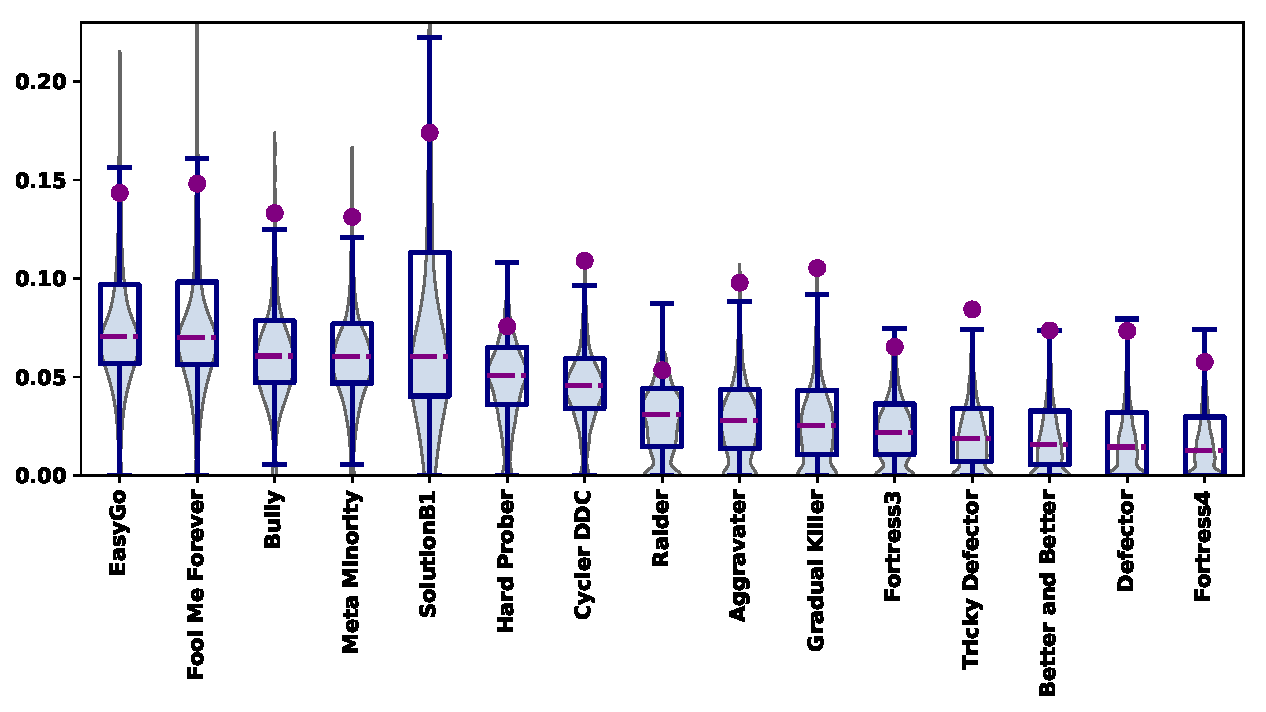
\includegraphics[width=.8\textwidth]{../images/performance_probend.pdf}
    \caption{\(\bar{r}\) distributions for best performed strategies in probabilistic ending tournaments.}
    \label{fig:probend_results}
\end{figure}

\subsection{Noisy \& probabilistic ending tournaments}\label{subsection:noisy_probend_tournament}

This section presents the results in tournaments that have both noise and an
unspecified number of turns. Several of the top ranked have been covered before
because they were highly ranked in noisy tournaments as well,
Table~\ref{table:noisy_prob_end_results}. However, strategies from the
top ranks of probabilistic ending tournaments did not rank highly here.

The Retaliates, $\phi, e$ and Anti Tit For Tat behaviour strategies appear to
perform well in noisy environments. So these strategies performed well in this
setting as well even though now the turns are not specified. The top ranked
strategy is Alternator a strategy that alternate between cooperation and
defection. Hopeless~\cite{Van2015} is a strategy that will only defect if and
only if a mutual cooperation and the last three places are occupied by
strategies based on a Q learning algorithm.

\begin{table}[!htbp]
    \centering
    \resizebox{.25\textwidth}{!}{
    \begin{tabular}{lr}
\toprule
Name                &                         $\bar{r}$    \\
\midrule
Alternator          &                                 0.30390 \\
$\phi$              &                                 0.31025 \\
$e$                 &                                 0.31293 \\
$\pi$               &                                 0.31818 \\
Limited Retaliate   &                                 0.35294 \\
Anti Tit For Tat    &                                 0.35429 \\
Retaliate 3         &                                 0.35484 \\
Limited Retaliate 3 &                                 0.35563 \\
Retaliate           &                                 0.35588 \\
Retaliate 2         &                                 0.35714 \\
Limited Retaliate 2 &                                 0.36066 \\
Hopeless            &                                 0.36913 \\
Arrogant QLearner   &                                 0.40526 \\
Cautious QLearner   &                                 0.40711 \\
Risky QLearner      &                                 0.41989 \\
\bottomrule
\end{tabular}
}
    \caption{Noisy and probabilistic ending top performances}\label{table:noisy_prob_end_results}
\end{table}

The three Q learning strategies are the only ones that have bimodal
distributions of normalised ranks similar to those of
Section~\ref{subsection:noisy_tournament}. In comparison, the rest of the
distributions are skewed towards 0.3 to 0.4
Figure~\ref{fig:noisy_probend_results}.

\begin{figure}[!htbp]
    \centering
    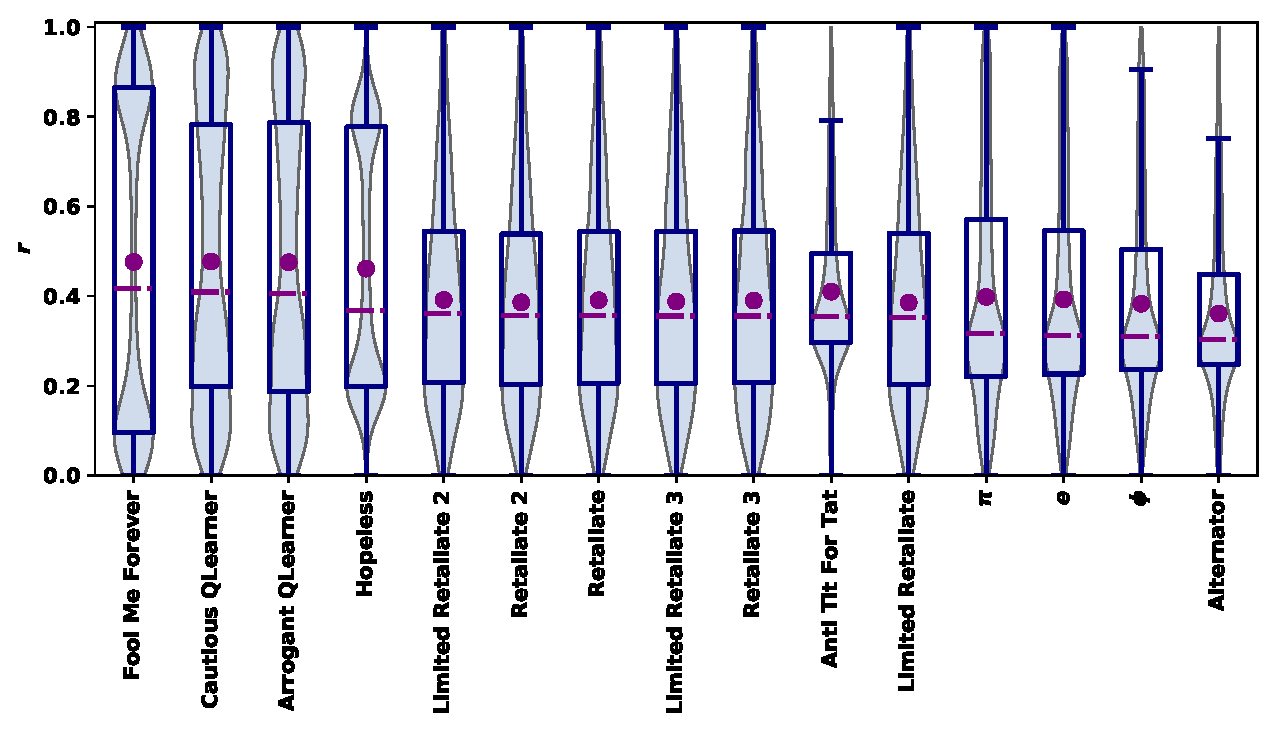
\includegraphics[width=.7\textwidth]{../images/performance_probend_noise.pdf}
    \caption{\(\bar{r}\) distributions for best performed strategies in noisy
    probabilistic ending tournaments.}
    \label{fig:noisy_probend_results}
\end{figure}

As yet, the performances of 186 different strategies have been evaluated in
four different tournaments. In standard tournaments the top ranked spots were
dominated by complex strategies that have been trained using reinforcement learning
techniques in a standard tournament. These strategies dominated most
the tournaments that have been involved in. In noisy tournaments the top ranked
strategies were all different to those of standard tournaments. Most of the
top ranked strategies have been strategies that were trying to keep the defections
and cooperations to a given ratio. These strategies had won most the tournaments
in which they participated, however, they also ranked last in several tournaments.
Once again in probabilistic ending tournaments the top ranked strategies were
different to those before. More defecting strategies occupied the top ranks
as well as finite state automata that have been introduced all by the same
authors. Finally, in noisy probabilistic ending tournaments it was the only
set of tournaments were the highly ranked strategies have been covered before,
more specifically, in noisy tournaments. However, in these tournaments the means
and medians of the distributions were close to 0.4. Indicating that on average
these strategies manage to beat only 60\% of the opponents.

In the following section the performance of the strategies is evaluated again
but this time the results of the tournament types are included in the
analysis.

\subsection{Top performance in data set}\label{subsrction:overall}

The data set described in Section~\ref{section:data_collection} contains results
from 49,140 tournaments and the performances in this section are 
based on these tournaments. The top ranked 15 strategies are given in
Table~\ref{table:overall_results}. It includes several strategies that have
ranked in the top spots in the separate tournament analysis.
The top spaces are overtaken by the Retaliate strategies, followed by BackStabber
and DoubleCrosser. DoubleCrosser is just an extension of BackStabber.
Nice Meta Winner and NMWE Memory One are strategies based on teams of strategies
and Stein and Rapoport and Grudger are strategies from Axelrod's original tournament
where they came 6th and 7th respectively. Forgetful Fool Me Once is a similar
strategy to Grudger but sometimes forgets and cooperates. Finally, both
PSO Gambler and Evolved HMM 5 are strategies introduced in~\cite{Harper2017}.

\begin{table}[!htbp]
    \centering
    \resizebox{.35\textwidth}{!}{
    \begin{tabular}{lr}
\toprule
{} &  Normalized\_Rank \\
Name                    &                  \\
\midrule
Evolved FSM 16          &            0.018 \\
Evolved HMM 5           &            0.019 \\
Evolved FSM 16 Noise 05 &            0.025 \\
EvolvedLookerUp2\_2\_2    &            0.028 \\
Evolved ANN             &            0.037 \\
PSO Gambler 2\_2\_2       &            0.040 \\
Evolved ANN 5           &            0.046 \\
PSO Gambler 1\_1\_1       &            0.061 \\
Fool Me Once            &            0.067 \\
Evolved FSM 4           &            0.075 \\
DoubleCrosser           &            0.079 \\
Winner12                &            0.081 \\
BackStabber             &            0.082 \\
DBS                     &            0.086 \\
PSO Gambler Mem1        &            0.089 \\
\bottomrule
\end{tabular}
}
    \caption{Top performances in data set}\label{table:overall_results}
\end{table}

The top ranked strategies include a good mixture of strategies. PSO Gambler and
Evolved HMM 5 are very complex strategies compared to Stein and Rapoport and
Grudger that are strategies manually designed. There are strategies based on
teams and the Retaliate strategies which have illustrated to do well in noise.
The Retaliates' distributions are very similar to each other,
Figure~\ref{fig:overall_results}, and different compared to the rest of the
distributions.

\begin{figure}[!htbp]
    \centering
    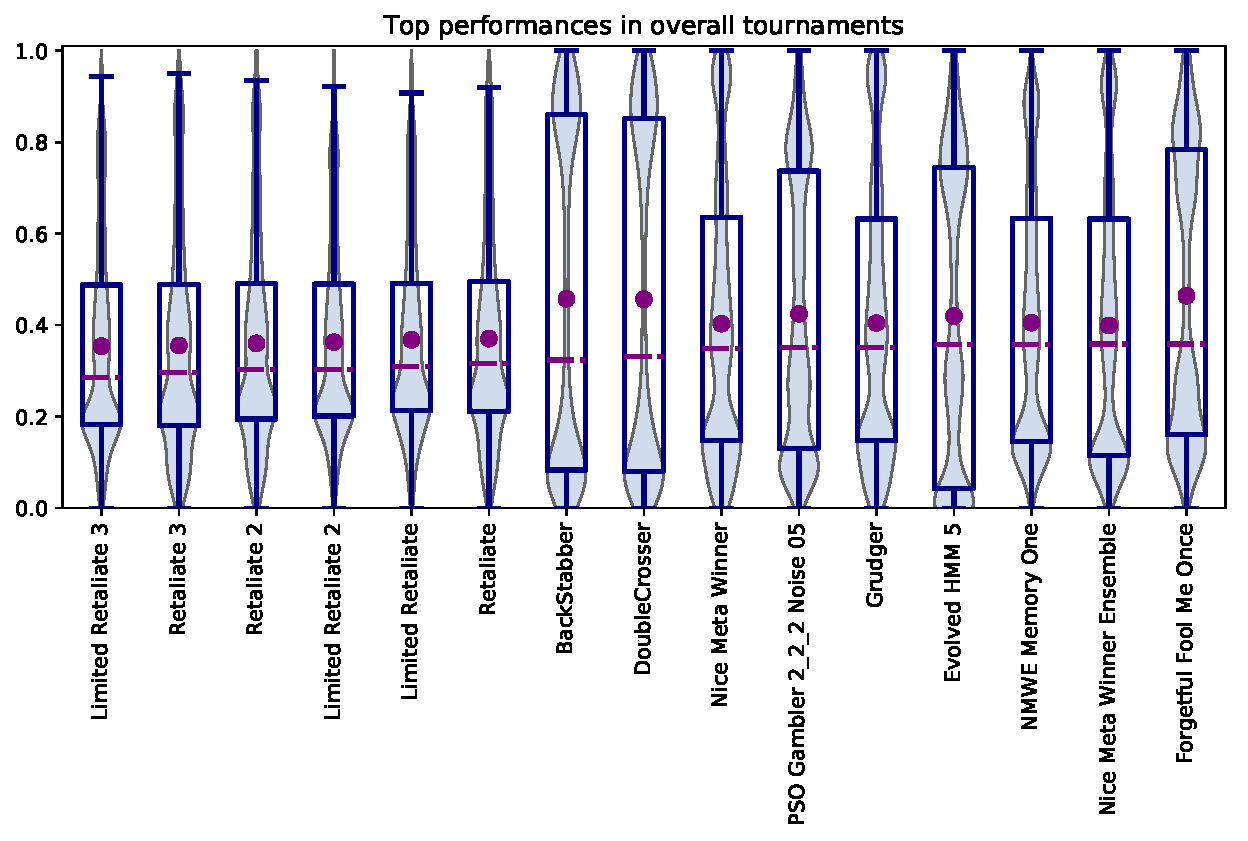
\includegraphics[width=.8\textwidth]{../images/performance_merged.pdf}
    \caption{\(\bar{r}\) distributions for best performed strategies in data set.}
    \label{fig:overall_results}
\end{figure}

However, are these strategies the answer as to how to play the IPD. The distributions
of their ranks are given for all the tournaments individually. Figure illustrates
that there are settings that these strategies perform well, that they perform
badly and settings that they perform average. Thus the conclusion is that there
is not a single dominant strategy in the IPD.


\begin{figure}[!htbp]
    \centering
    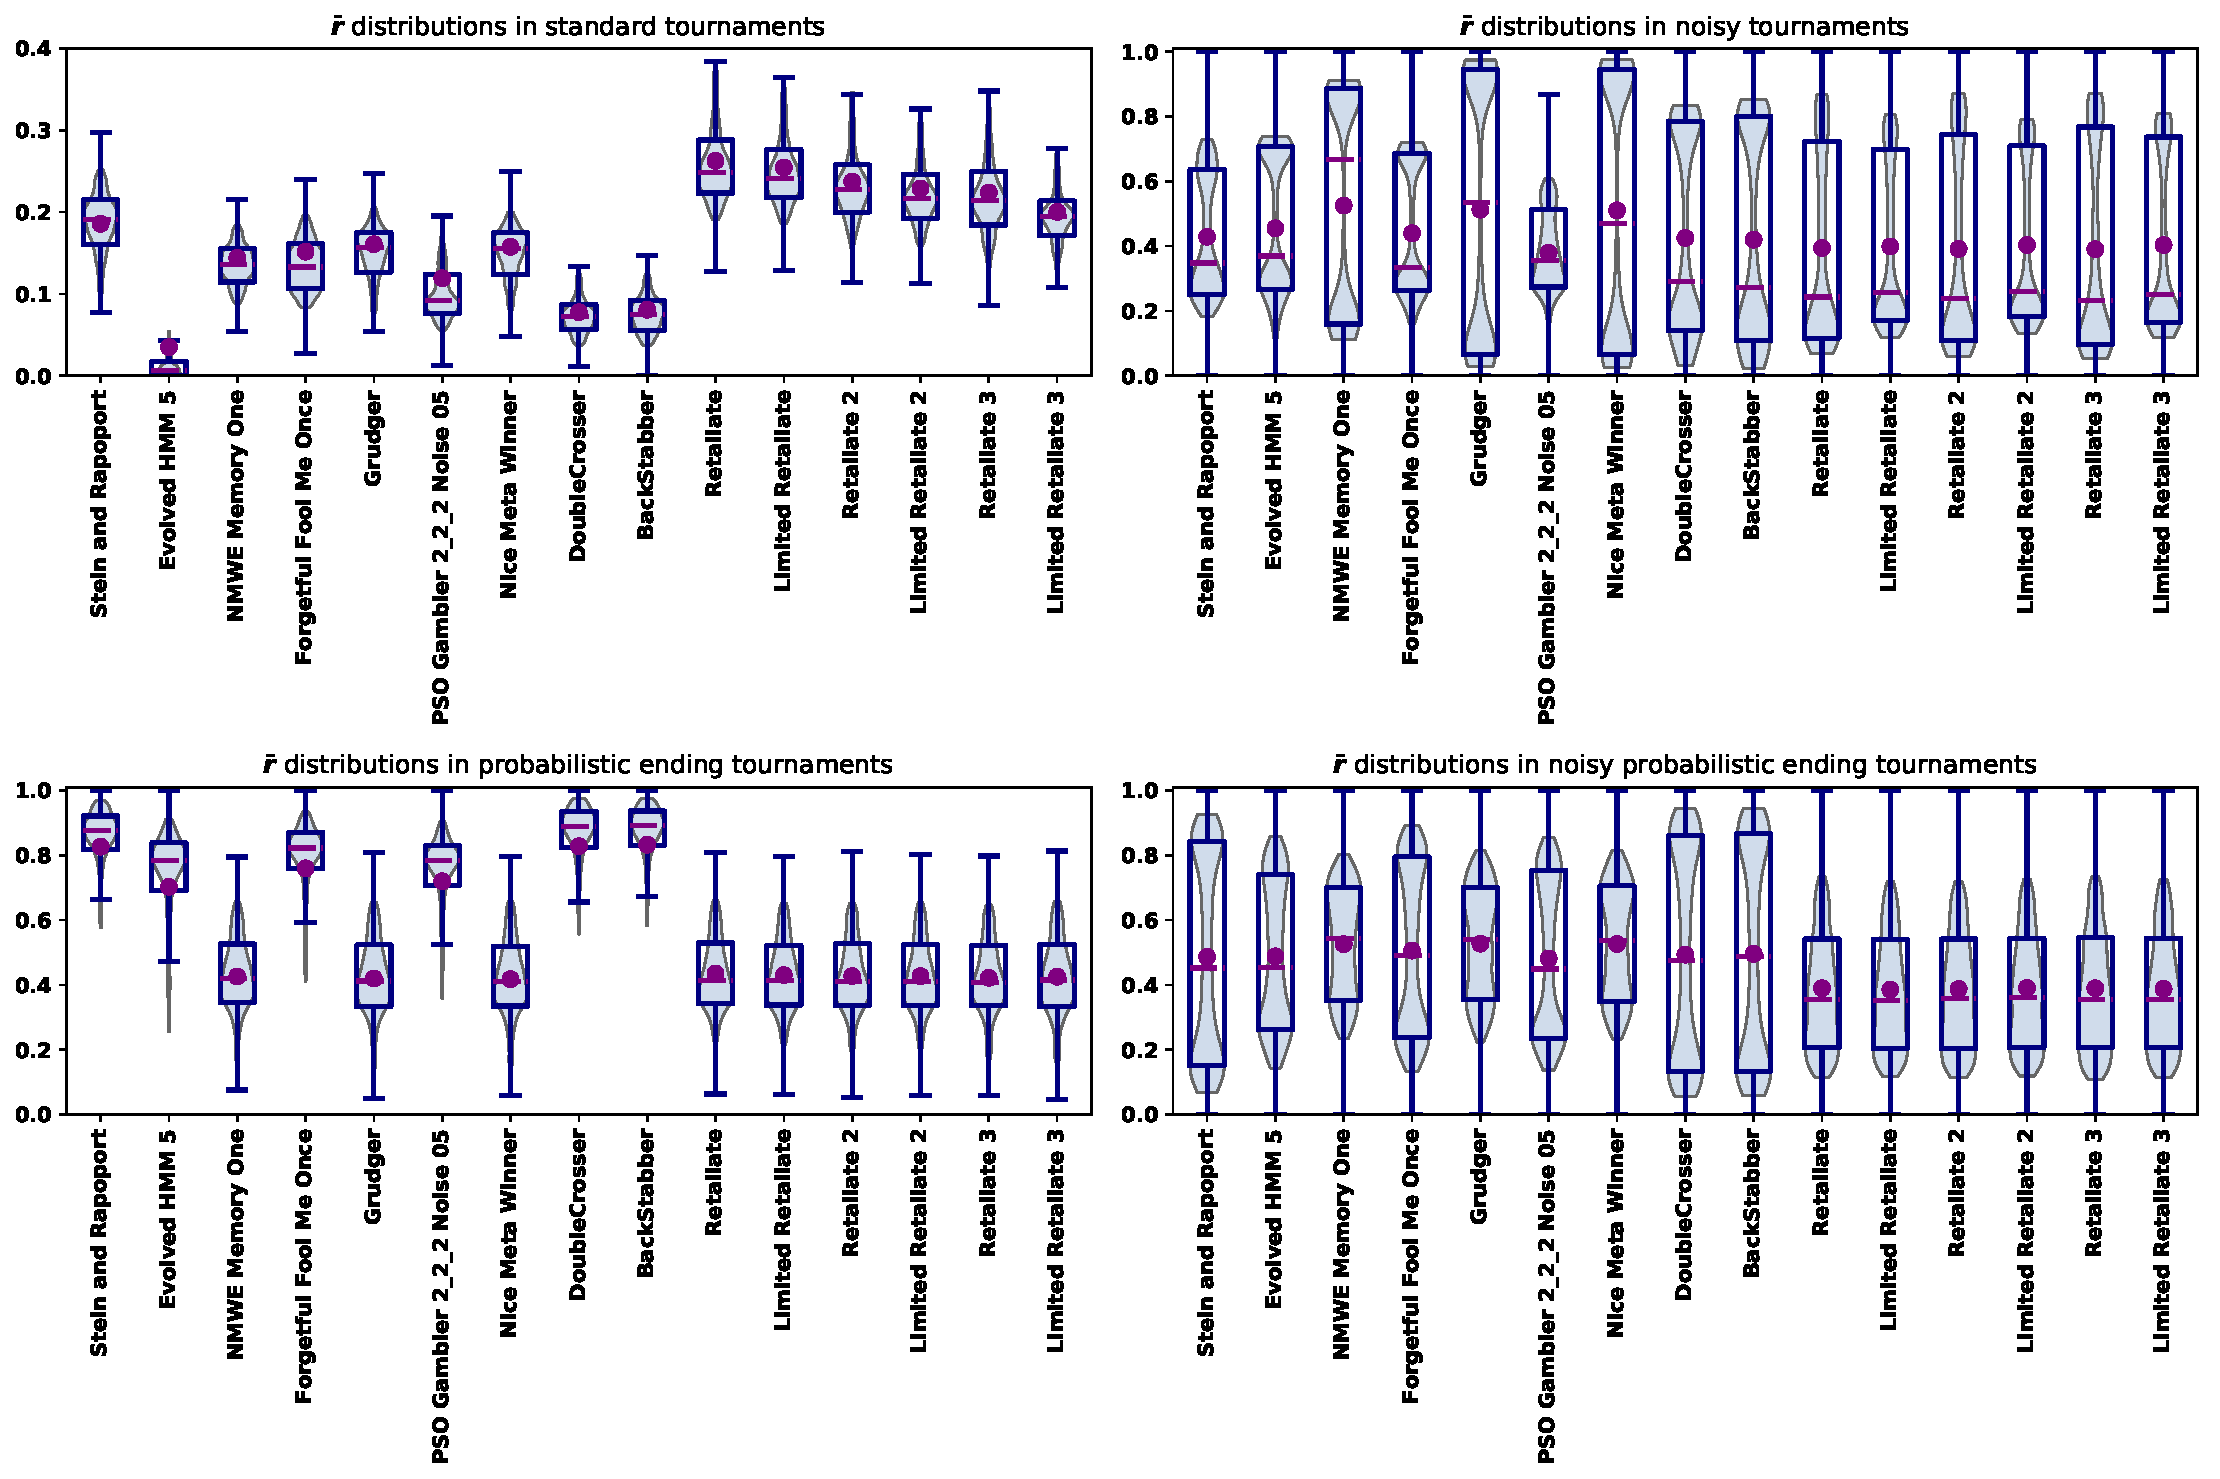
\includegraphics[width=.8\textwidth]{../images/performance.pdf}
    \caption{\(\bar{r}\) distributions for best performed strategies in data set.}
    \label{fig:overall_results}
\end{figure}


In this section the top ranked performances were presented. This was not done in
a single tournament of a given list of opponents, as many in the literature, but
over a number of tournaments where the list and size could vary. Moreover, four
different type of tournaments were performed in this work. Even with the large
number of tournaments there some think that is evident, there is not a single
best strategy. Though some strategies seem to be repeated, there are other
tournament types that they are not. The top ranks are occupied but almost
different strategies every time. And in the top spots the strategies behaviour
differ. There are simple and complex, with small memory and large, deterministic
and stochastic. Is there a single dominant strategy in the iterated prisoner's
dilemma? We argue not.

The aim of the next section is to understand which are the factors that made
these strategies successful. In each setting separately but also overall.

\section{Evaluation of performance}\label{section:evaluation_of_performance}

This section explores the factors that contributed to the successful performance
of strategies described in Section~\ref{section:top_performances}.
The factors
evaluated in this work are given by Table~\ref{table:manual_measures}. Several
of these factors include measures regarding the strategies and it's behaviour
however others are fixed from the tournament or even the type of tournament. The
measures from Table 1 are also included.



This is achieved by
separating the strategies performances into successful ones and non. The performances
are separated on the normalised rank and the median score using the clustering
algorithm \(k-\)means~\cite{Arthur2007}. The number of clusters is not deterministic
but the decision is based on the silhouette coefficients~\cite{Rousseeuw1987}.

Consider the performances in the standard tournaments.
Figure~\ref{fig:standard_clusters} gives the normalised rank against the median
score for three trials of the clustering algorithm with number of clusters being
2, 3 and 4. A number of 2 clusters gives the highest silhouette coefficient (0.66)
and so it's selected for the standard tournaments. More specifically,
being in cluster 1 corresponds to a low performance whereas being in cluster
2 corresponds to a high performance. These are based on the median normalised
rank and median score of each cluster as shown in Table~\ref{table:clusters}.

\begin{figure}[!htbp]
    \centering
    \includegraphics[width=.7\textwidth]{../output/standard/clusters_plots.png}
    \caption{Clustering trials for standard tournaments. A number of 2
    clusters has been chosen with a silhouette score of  0.66 against 0.511 and 0.50
    respectively.}\label{fig:standard_clusters}
\end{figure}

\begin{table}[!htbp]
    \centering
    \resizebox{.25\textwidth}{!}{
    \begin{tabular}{lcc}
    \toprule
    Cluster                &   $\bar{r}$ & median score \\
    \midrule
    1 & 0.769 & 2.065 \\
    2 & 0.263 & 2.639\\
    \bottomrule
    \end{tabular}}
    \caption{Median normalised rank and median score of each cluster in standard tournaments.}
    \label{table:clusters}
\end{table}

Now that the performances have been clustered the aim is to evaluate which
factors affect the performances being in each respective cluster. The factors
evaluated in this work are given by Table~\ref{table:manual_measures}. Several
of these factors include measures regarding the strategies and it's behaviour
however others are fixed from the tournament or even the type of tournament. The
measures from Table 1 are also included.

\newcolumntype{g}{>{\columncolor{Gray}}c}
\begin{table}[h]
    \begin{center}
    \resizebox{\textwidth}{!}{
    \begin{tabular}{gcgcgc}
    \toprule
    measure & measure explanation &  source & value type & min value & max value \\
    \midrule
stochastic  &  If a strategy is stochastic & strategy classifier from~\cite{axelrodproject} & boolean  & False &  True \\
makes use of game &  If a strategy makes used of the game information & strategy classifier from~\cite{axelrodproject} & boolean  & False &  True \\
makes use of length &  If a strategy makes used of the number of turns & strategy classifier from~\cite{axelrodproject} & boolean  & False &  True \\
SSE & A measure of how far a strategy is from extortionate behaviour & method described in~\cite{Knight2019} & float & 0 & 1 \\
max cooperating rate $(C_{\text{max}})$  & The biggest cooperating rate in the tournament & result summary & float & 0 & 1 \\
min cooperating rate $(C_{\text{min}})$ & The smallest cooperating rate in the tournament & result summary & float & 0 & 1 \\
median cooperating rate $(C_{\text{median}})$ & The median cooperating rate in the tournament & result summary & float & 0 & 1 \\
mean cooperating rate $(C_{\text{mean}})$ & The mean cooperating rate in the tournament & result summary & float & 0 & 1 \\
$C_r$ / $C_{\text{max}}$ & A strategy's cooperating rate divided by the maximum & manually & float & 0 & 1 \\
$C_r$ / $C_{\text{min}}$ & A strategy's cooperating rate divided by the minimum & manually & float & 0 & 1 \\
$C_r$ / $C_{\text{median}}$ & A strategy's cooperating rate divided by the median & manually & float & 0 & 1 \\
$C_r$ / $C_{\text{mean}}$ & A strategy's cooperating rate divided by the mean & manually & float & 0 & 1 \\
$CC$ to $C$ rate & The probability a strategy will cooperate after a mutual cooperation & result summary & float & 0 & 1 \\
$CD$ to $C$ rate & The probability a strategy will cooperate after being betrayed by the opponent & result summary & float & 0 & 1 \\
$DC$ to $C$ rate & The probability a strategy will cooperate after betraying the opponent & result summary & float & 0 & 1 \\
$DD$ to $C$ rate & The probability a strategy will cooperate after a mutual defection & result summary & float & 0 & 1 \\
    \bottomrule
        \end{tabular}}
    \end{center}
    \caption{Manually calculated/retrieved measures.}
    \label{table:manual_measures}
\end{table}

%memory depth &  Strategy's memory size & strategy classifier from~\cite{axelrodproject} & integer & 0 & $\infty$ \\

To evaluated how significant each factor contribution was a random forest is
applied to the performances of standard tournaments where the target value
is their corresponding cluster. Figure~\ref{fig:importance_standard} gives the
importance of each factor.
The four factors that have affect more the performances of strategies
in standard tournaments are the cooperation ratio compared to the mean, the SSE,
the cooperation ratio compared to the median and the cooperating ratio after
being betrayed by the opponent.

\begin{figure}
    \begin{minipage}{.5\textwidth}
        \centering
        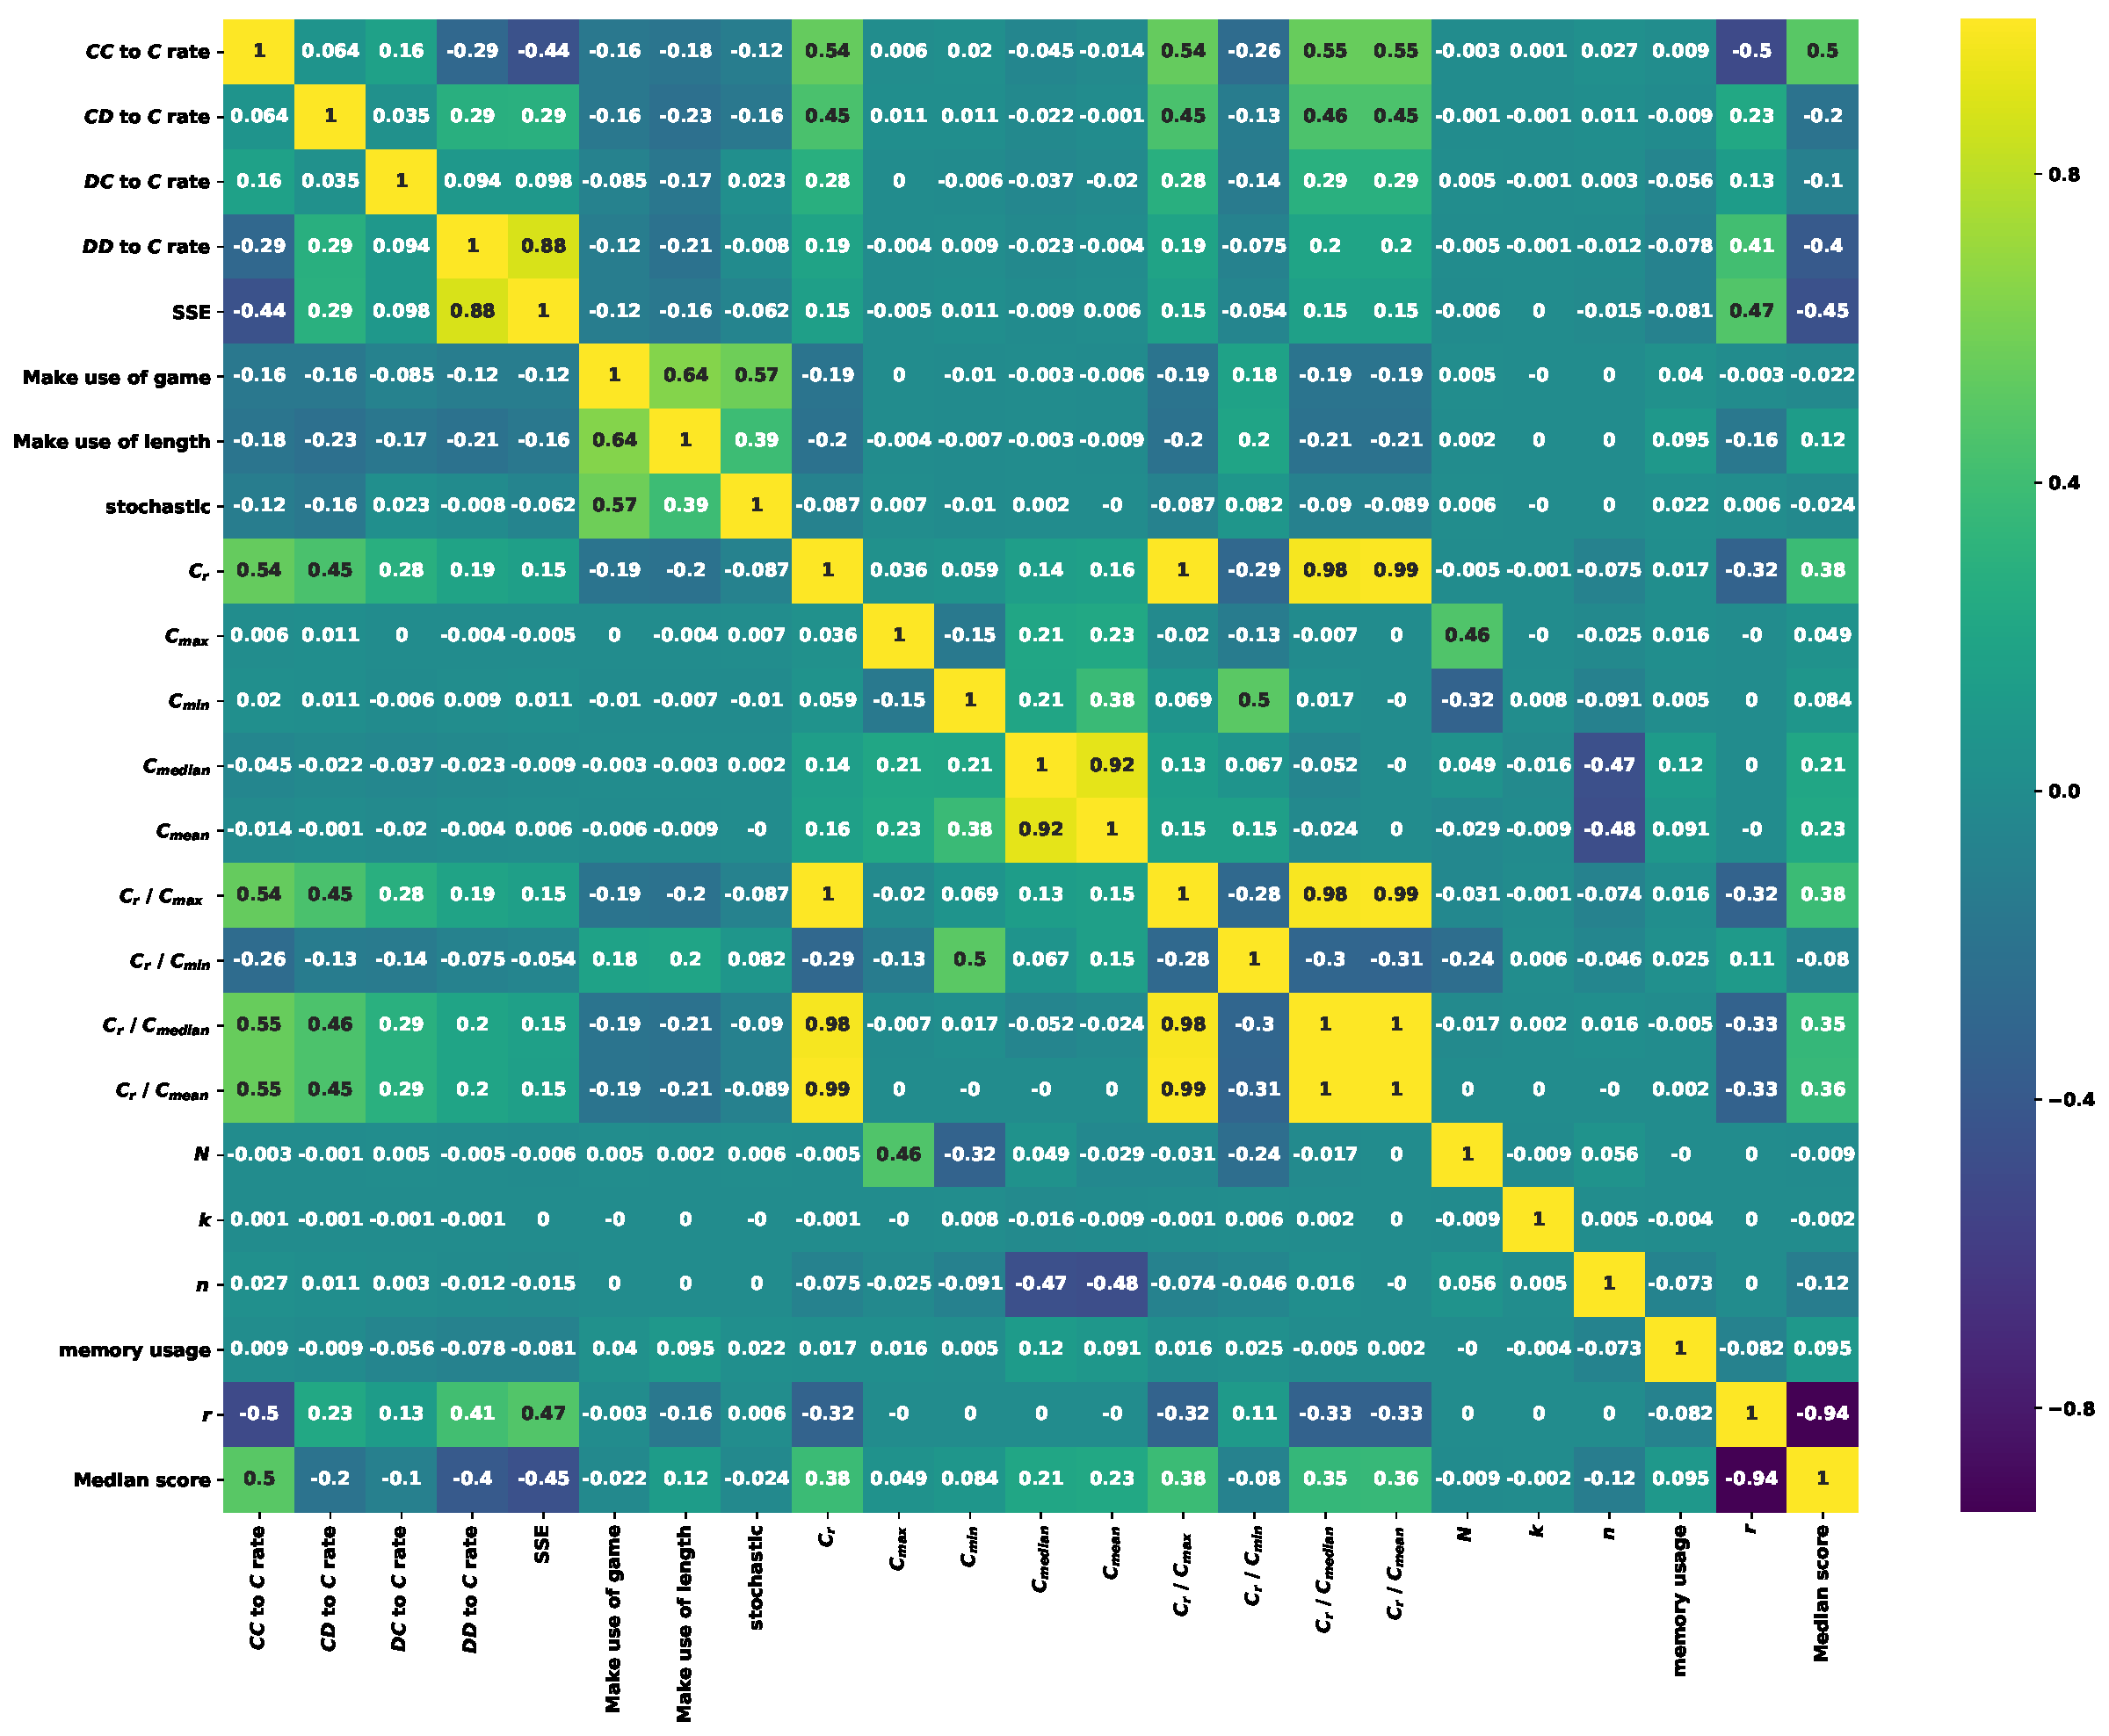
\includegraphics[width=\textwidth]{../images/standard_correlation_plot.pdf}
    \end{minipage}
    \begin{minipage}{.5\textwidth}
        \centering
        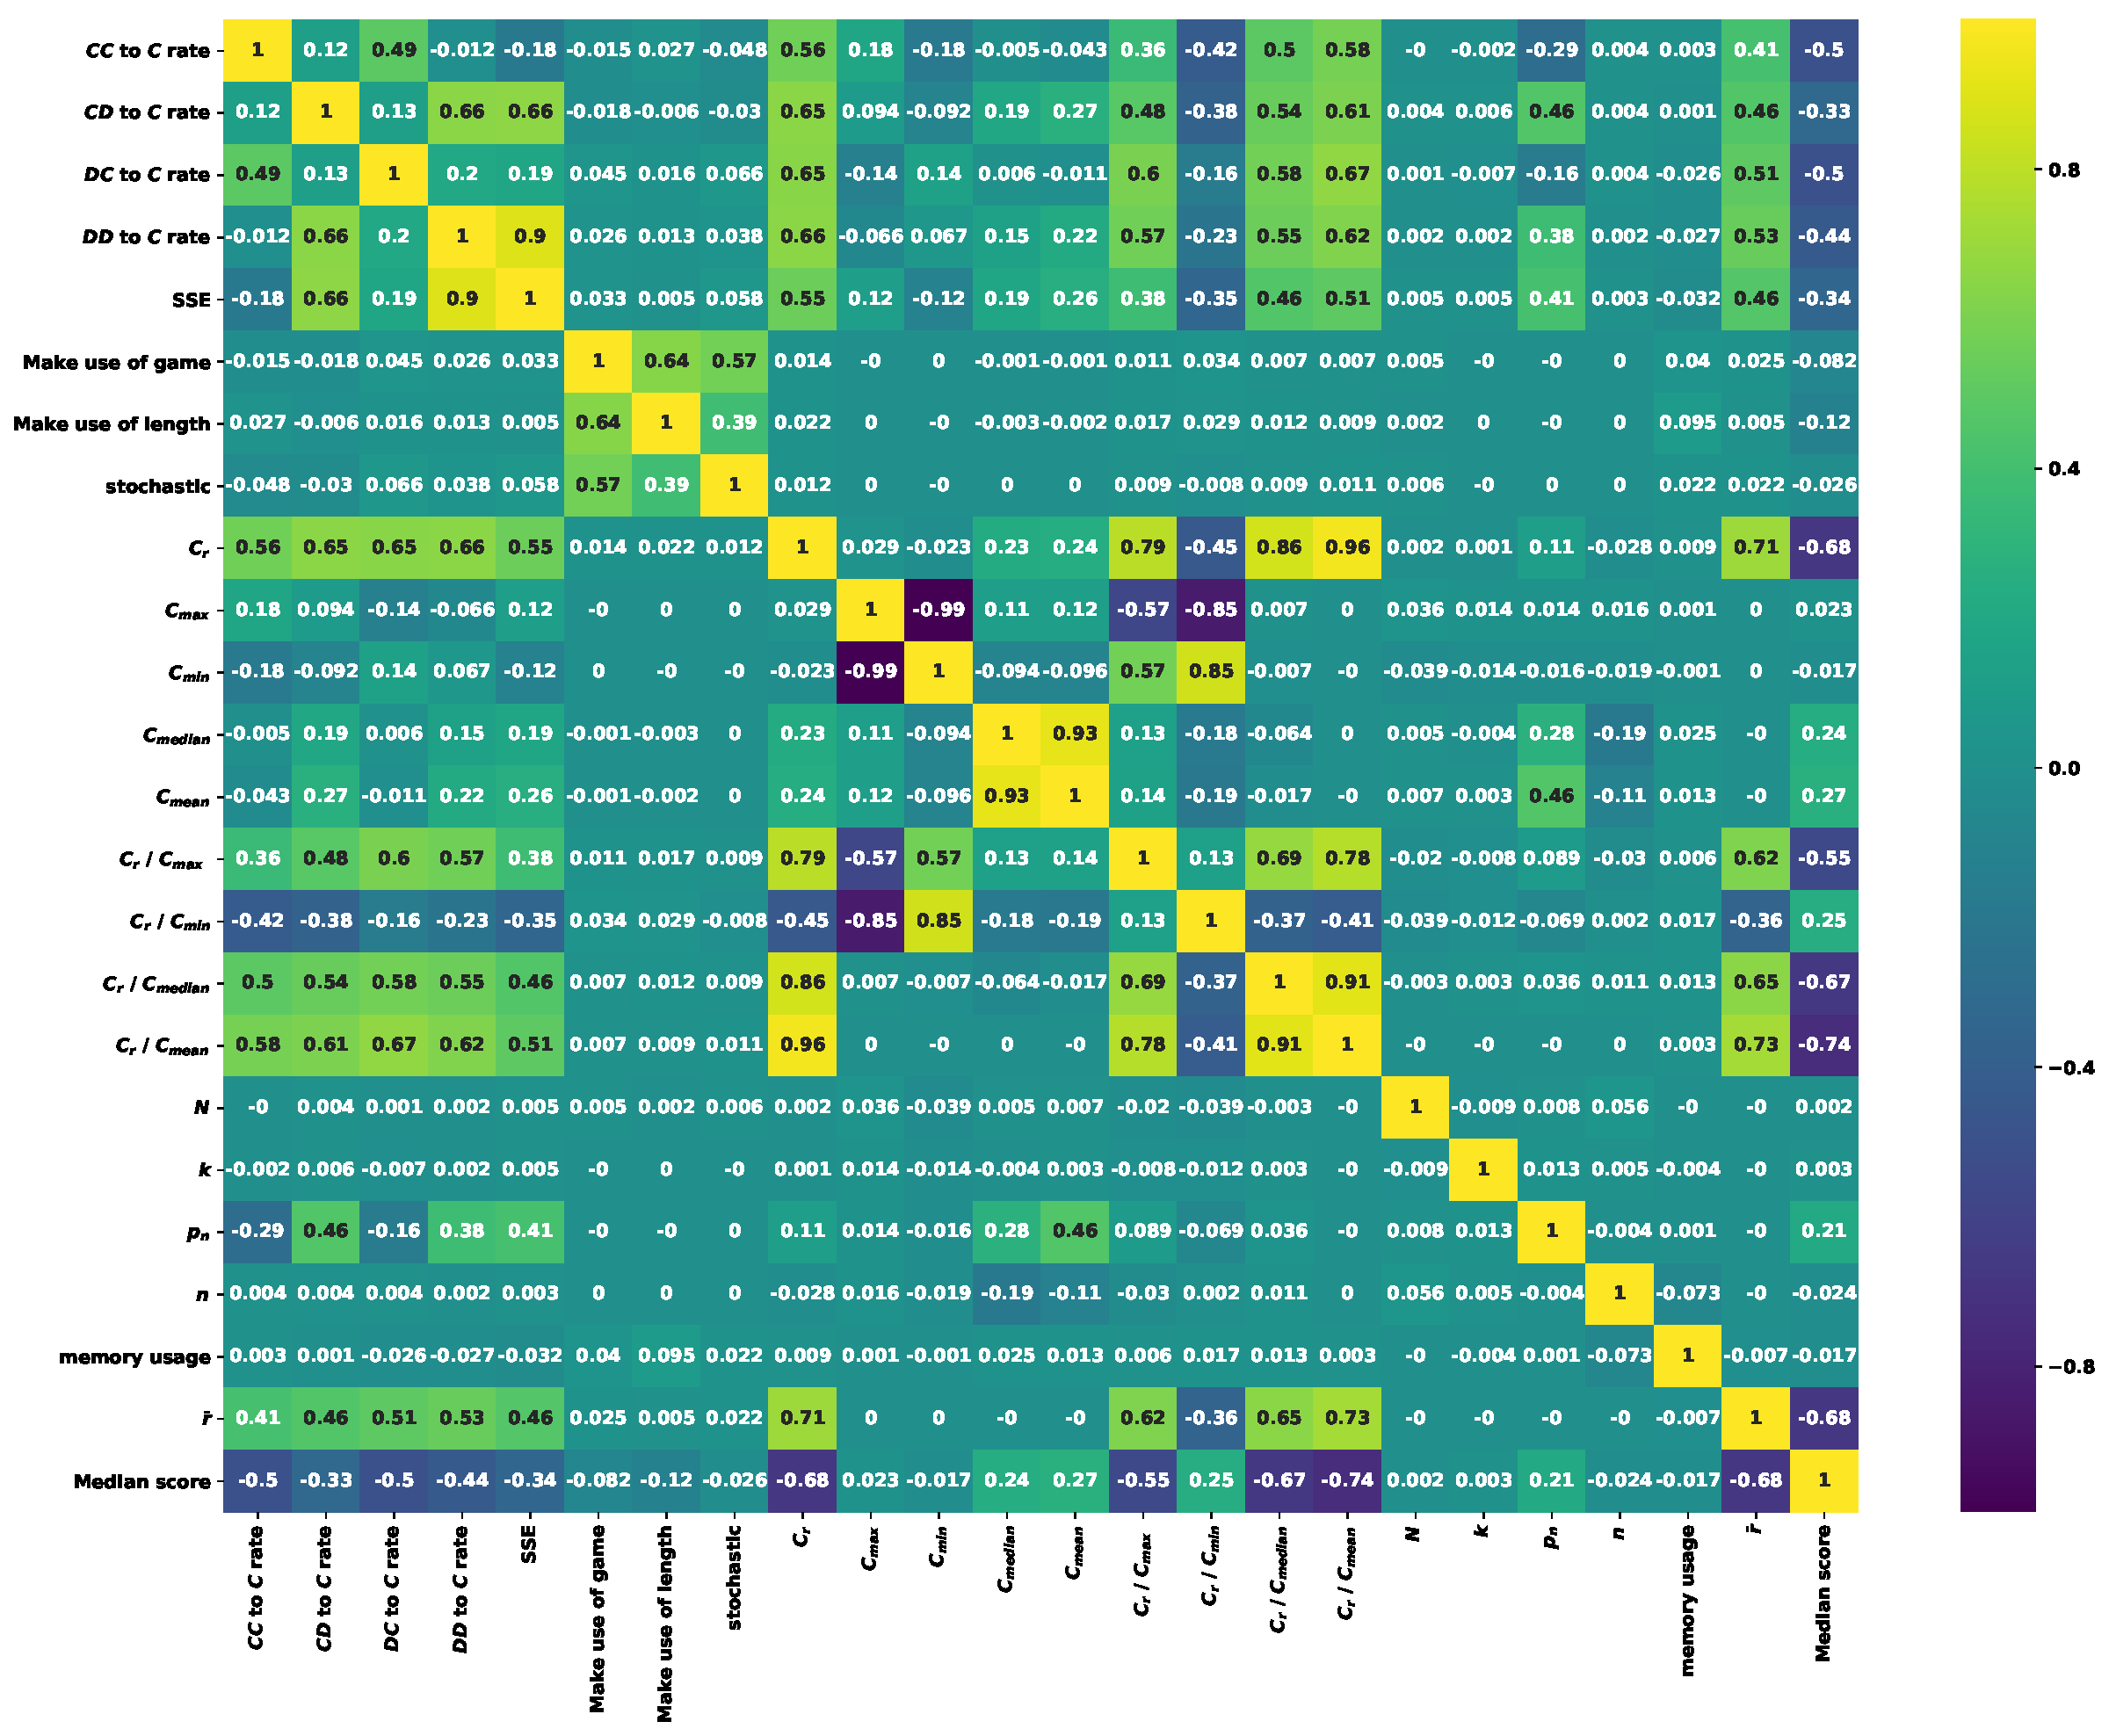
\includegraphics[width=\textwidth]{../images/noise_correlation_plot.pdf}
    \end{minipage}
    \begin{minipage}{.5\textwidth}
        \centering
        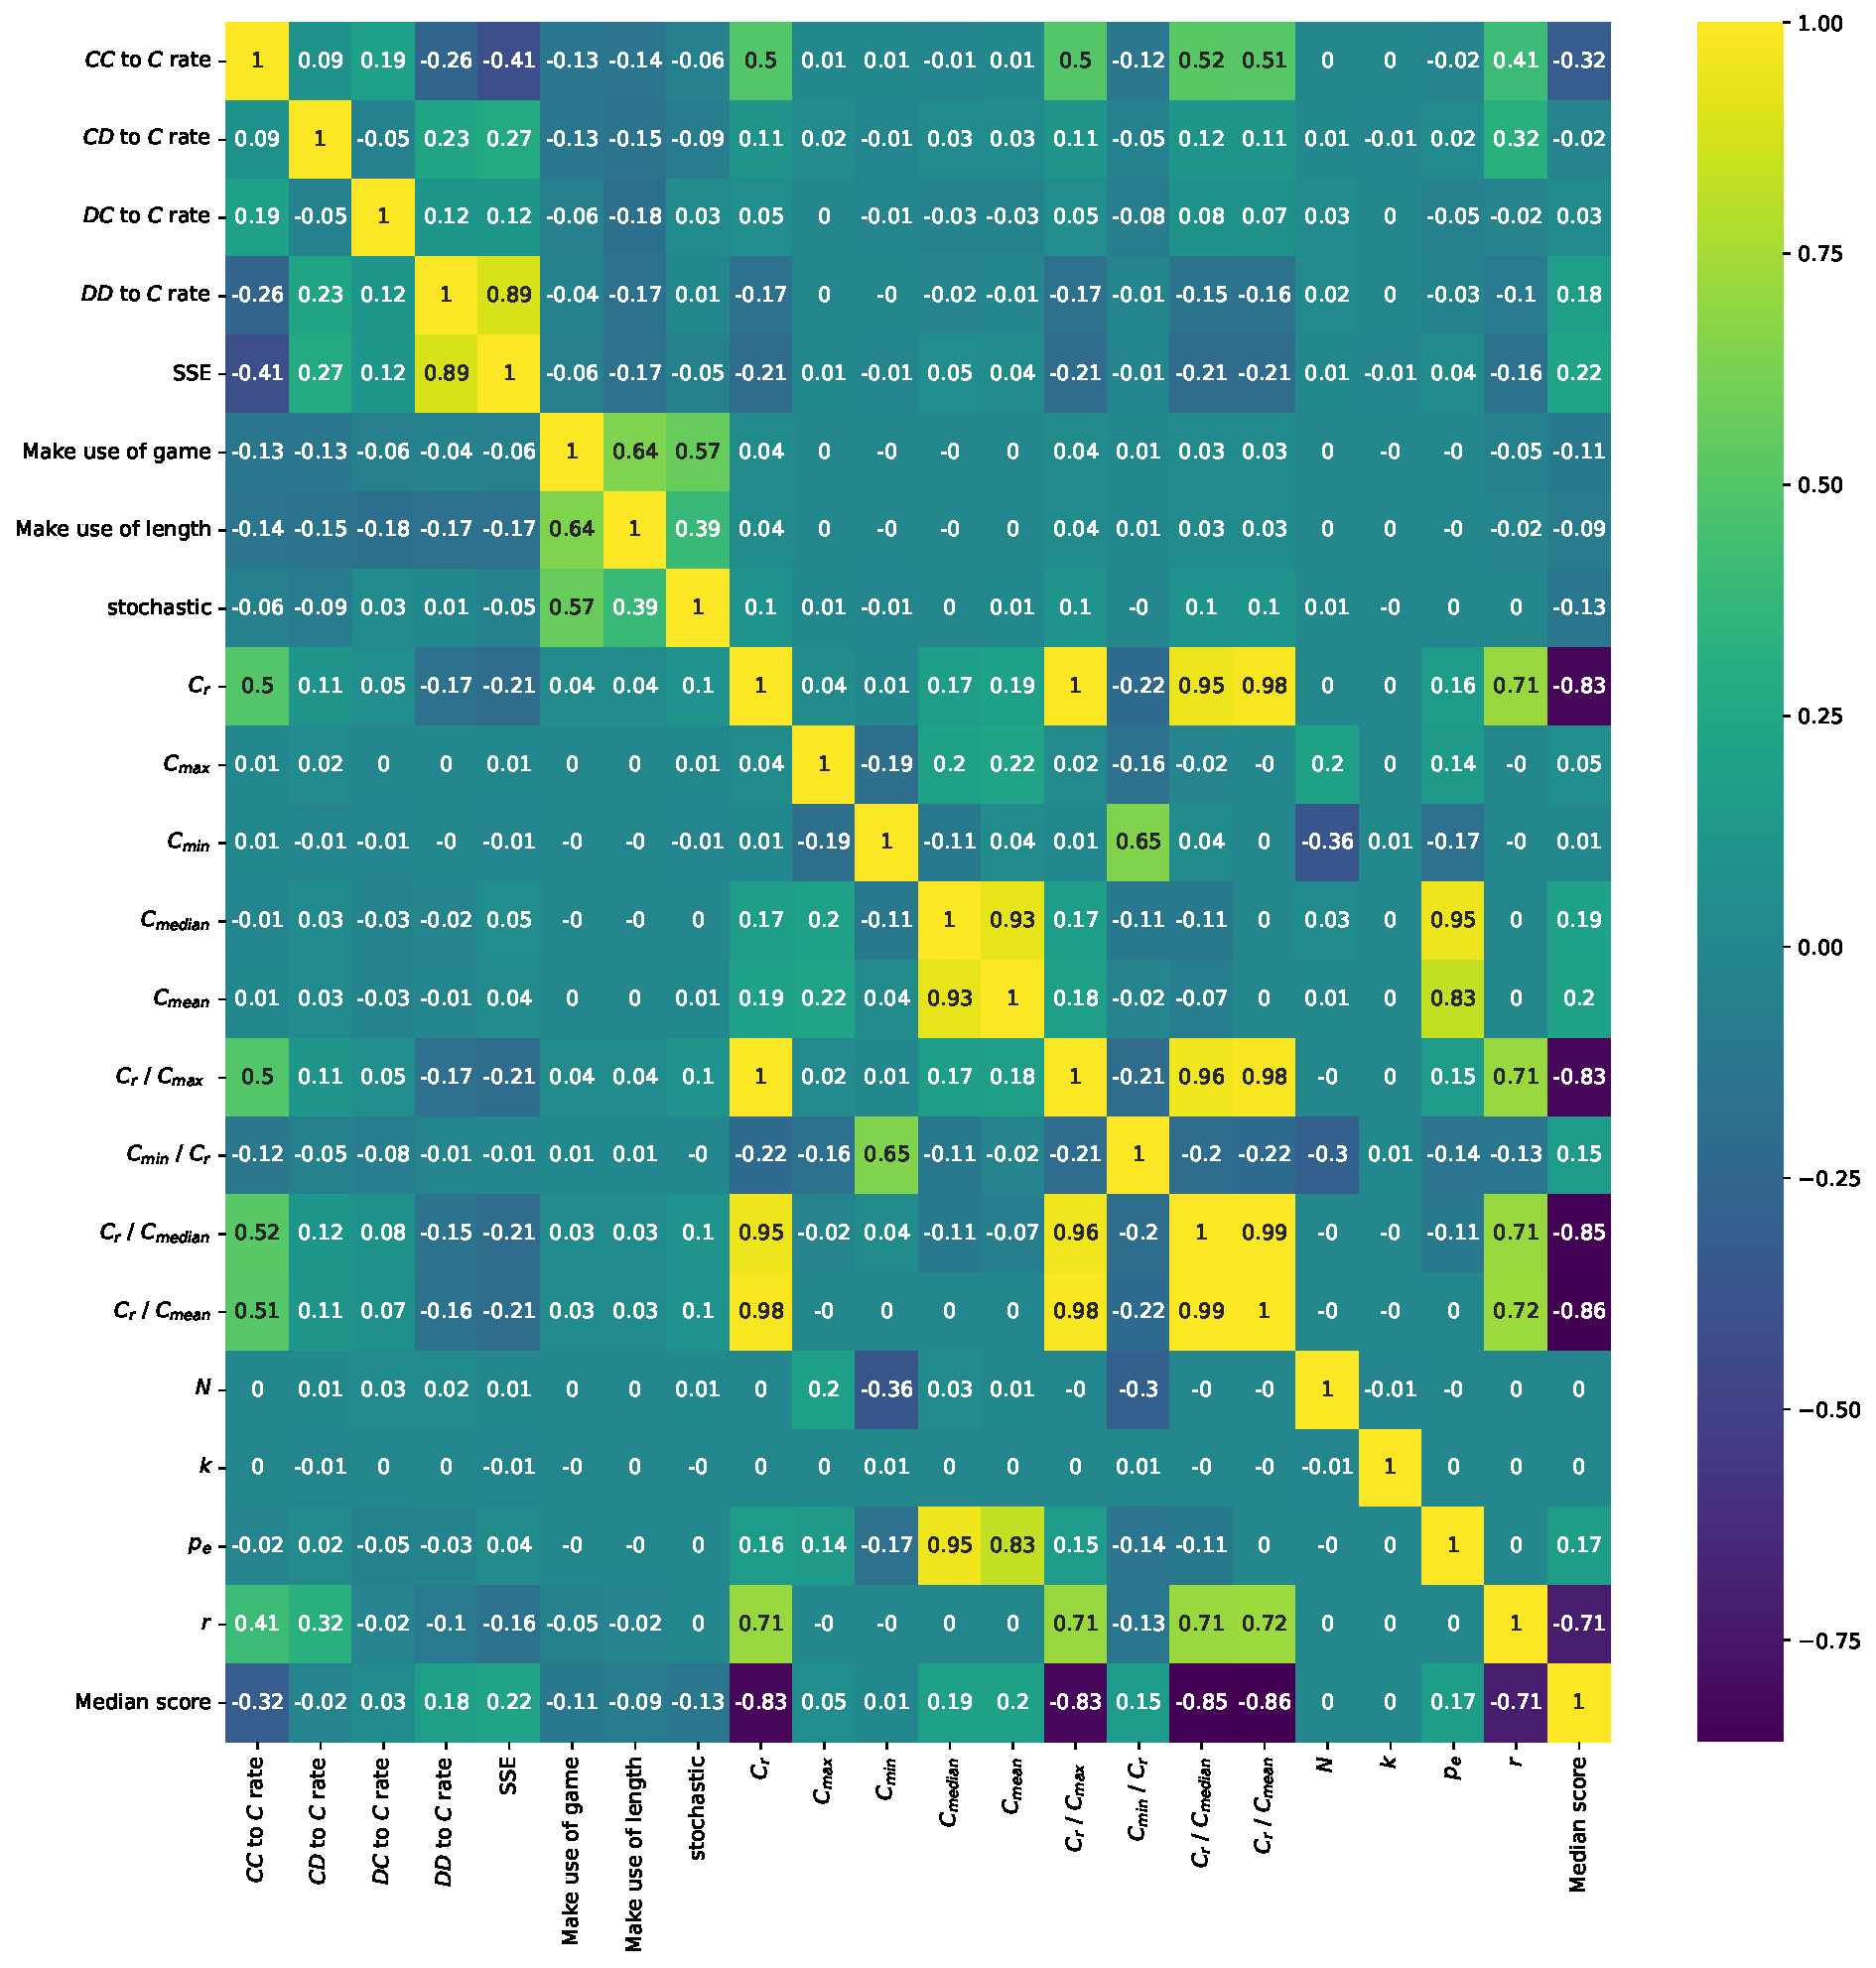
\includegraphics[width=\textwidth]{../images/probend_correlation_plot.pdf}
    \end{minipage}
    \begin{minipage}{.5\textwidth}
        \centering
        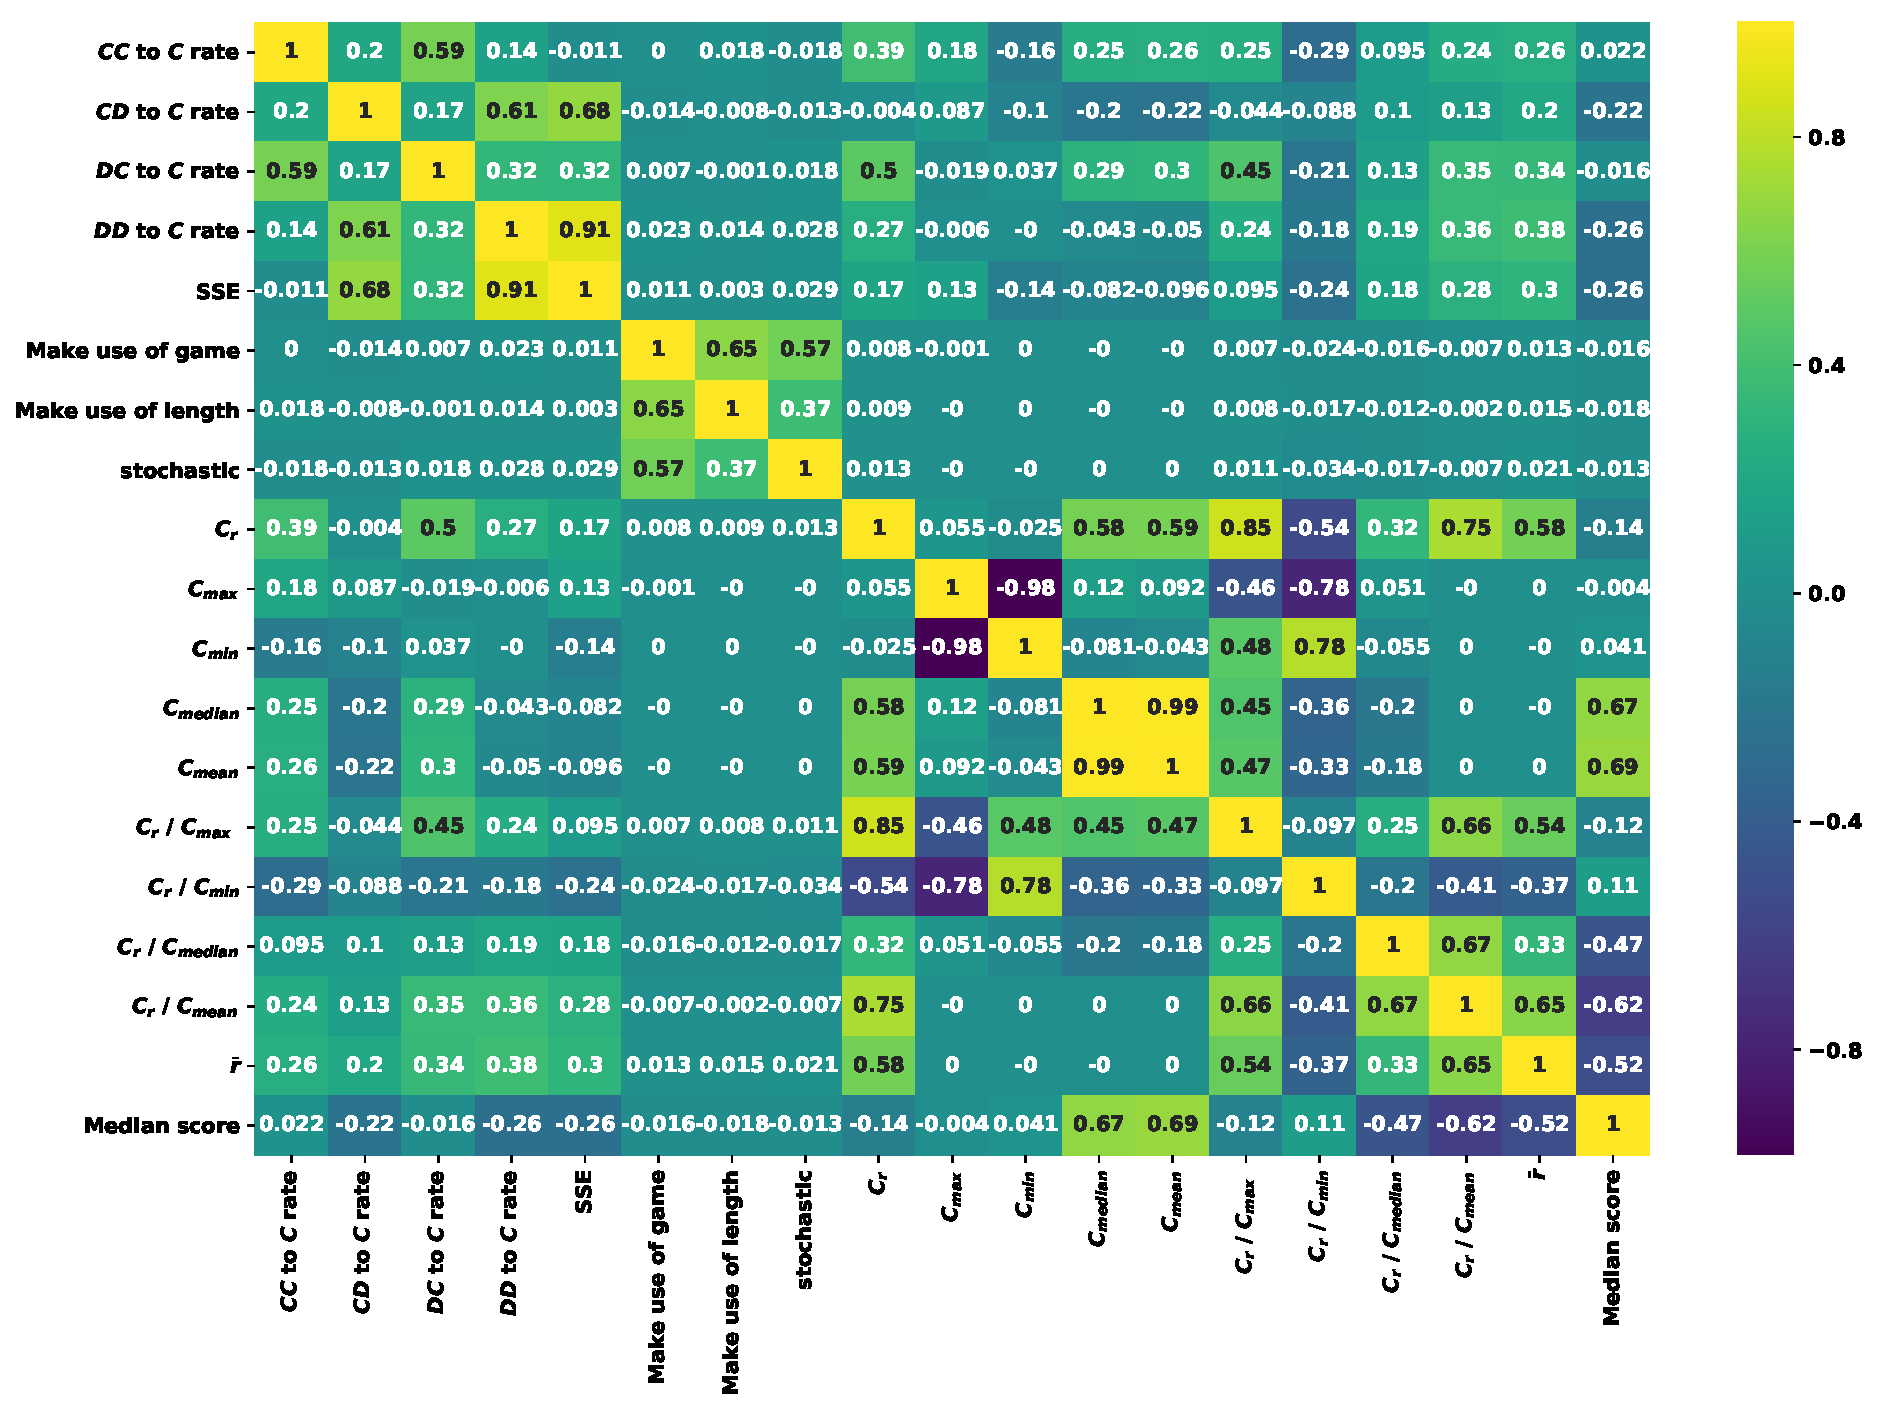
\includegraphics[width=\textwidth]{../images/probend_noise_correlation_plot.pdf}
    \end{minipage}
\end{figure}


To delved deeper into the results of the random forest and how each feature
has helped to be clustered where you were the tree interpreter method
described in~\cite{} is used. The strongest contributors to predicting that
a performance was clustered in the successful class were the DC to D ratio,
the SSE error, the size followed by the cooperating ratio compared to the mean.
In comparison the strongest impact on being in the non successful cluster
have the Cd to C rate and the cooperating ration compare to the median.

\begin{figure}[!htbp]
    \begin{minipage}{.6\textwidth}
    \centering
    \includegraphics[width=\textwidth]{../output/standard/_feature_importance_bar_plot.pdf}
    \caption{Importance of features in standard tournaments.}
    \label{fig:importance_standard}
    \end{minipage}\hspace{.1cm}
    \begin{minipage}{.35\textwidth}
        \vspace{-1.5cm}
        \centering
        \resizebox{1.1\textwidth}{!}{
        \begin{tabular}{lrrr}
\toprule
{} &  importance &  cluster 1 &  cluster 2 \\
\midrule
$DC$ to $C$ rate     &    0.042803 &  -0.000321 &   0.000321 \\
SSE                  &    0.163466 &  -0.000317 &   0.000317 \\
$n$                  &    0.021574 &  -0.000159 &   0.000159 \\
$C_r$ / $C_{mean}$   &    0.170318 &  -0.000112 &   0.000112 \\
$CC$ to $C$ rate     &    0.072634 &  -0.000091 &   0.000091 \\
stochastic           &    0.004977 &  -0.000064 &   0.000064 \\
$C_{min}$            &    0.003700 &  -0.000037 &   0.000037 \\
$C_{mean}$           &    0.010065 &  -0.000031 &   0.000031 \\
$C_r$ / $C_{min}$    &    0.004783 &  -0.000022 &   0.000022 \\
Make use of length   &    0.002762 &  -0.000016 &   0.000016 \\
Make use of game     &    0.003964 &  -0.000002 &   0.000002 \\
$C_r$ / $C_{max}$    &    0.072897 &   0.000028 &  -0.000028 \\
$C_{median}$         &    0.015318 &   0.000028 &  -0.000028 \\
$C_{max}$            &    0.003928 &   0.000033 &  -0.000033 \\
$DD$ to $C$ rate     &    0.050942 &   0.000062 &  -0.000062 \\
$C_r$                &    0.063826 &   0.000088 &  -0.000088 \\
$CD$ to $C$ rate     &    0.132096 &   0.000277 &  -0.000277 \\
$C_r$ / $C_{median}$ &    0.159947 &   0.000346 &  -0.000346 \\
\bottomrule
\end{tabular}
}
        \caption{The average contribution of each factor in standard tournaments
        based on the tree interpreter method.}
    \end{minipage}
\end{figure}

The same approach is applied to the tournament types individually and in the
merged performances fom the the tournament types. More specifically, in noisy
tournament the normalised rank against the median score is given in
Figure~\ref{fig:noise_clusters}, based on the silhouette coefficient the number
of clusters is 3 in noisy tournaments. The performance of each cluster is
a follows, being in cluster 1 corresponds to low performance, 2 in medium
and 3 high, Table~\ref{table:clusters_noisy}.

\begin{figure}[!htbp]
    \centering
    \includegraphics[width=.7\textwidth]{../output/noise/clusters_plots.png}
    \caption{Clustering trials for noisy tournaments. A number of 3
    clusters has been chosen with a silhouette score of 0.49 against 2 clusters
    with a coefficient of 0.47 and 4 with 0.45.
    respectively.}\label{fig:noise_clusters}
\end{figure}

\begin{table}[!htbp]
    \centering
    \resizebox{.25\textwidth}{!}{
    \begin{tabular}{lcc}
    \toprule
    Cluster                &   $\bar{r}$ & median score \\
    \midrule
    1 & 0.788 & 2.096 \\
    2 & 0.316 & 2.290 \\
    3 & 0.097 & 3.012 \\
    \bottomrule
    \end{tabular}}
    \caption{Median normalised rank and median score of each cluster in noisy tournaments.}
    \label{table:clusters_noisy}
\end{table}

The two factor that appear to affect the performance in noisy tournaments, based on the
average importance, are the cooperating ratio compared to the mean and the mean (Figure~\ref{fig:importance_noisy})
with both having a strong effect to the contribution of being in the successful
cluster Table~\ref{table:tree_interpreter_noise}.

\begin{figure}[!htbp]
    \begin{minipage}{.6\textwidth}
    \centering
    \includegraphics[width=\textwidth]{../output/noise/_feature_importance_bar_plot.pdf}
    \caption{Importance of factors from Table 8 in noisy tournaments.}
    \label{fig:importance_noisy}
    \end{minipage}\hspace{.1cm}
    \begin{minipage}{.35\textwidth}
        \vspace{-1.5cm}
        \centering
        \resizebox{1.2\textwidth}{!}{
        \begin{tabular}{lrrrr}
\toprule
{} &  importance &  cluster 1 &  cluster 2 &  cluster 3 \\
\midrule
$C_r$ / $C_{mean}$   &     0.21004 &   -0.00025 &    0.00008 &    0.00017 \\
$C_r$ / $C_{median}$ &     0.19222 &    0.00029 &   -0.00044 &    0.00015 \\
$C_{median}$         &     0.03806 &    0.00005 &   -0.00014 &    0.00009 \\
$p$                  &     0.07831 &    0.00000 &   -0.00008 &    0.00008 \\
$C_r$ / $C_{max}$    &     0.06782 &    0.00008 &   -0.00016 &    0.00008 \\
SSE                  &     0.05214 &   -0.00002 &   -0.00003 &    0.00005 \\
$DD$ to $C$ rate     &     0.04593 &   -0.00010 &    0.00006 &    0.00004 \\
$n$                  &     0.01400 &   -0.00002 &   -0.00002 &    0.00004 \\
$DC$ to $C$ rate     &     0.10295 &   -0.00042 &    0.00041 &    0.00001 \\
$C_{max}$            &     0.01509 &    0.00006 &   -0.00007 &    0.00001 \\
$C_r$ / $C_{min}$    &     0.02130 &    0.00003 &   -0.00003 &    0.00000 \\
stochastic           &     0.00367 &    0.00001 &   -0.00001 &    0.00000 \\
Make use of game     &     0.00175 &    0.00005 &   -0.00003 &   -0.00001 \\
$C_r$                &     0.03979 &    0.00015 &   -0.00014 &   -0.00001 \\
$C_{min}$            &     0.01823 &    0.00009 &   -0.00005 &   -0.00004 \\
$CC$ to $C$ rate     &     0.03104 &    0.00005 &    0.00001 &   -0.00006 \\
Make use of length   &     0.00685 &    0.00004 &    0.00004 &   -0.00008 \\
$C_{mean}$           &     0.03081 &    0.00007 &    0.00002 &   -0.00009 \\
$CD$ to $C$ rate     &     0.03000 &    0.00013 &    0.00001 &   -0.00014 \\
\bottomrule
\end{tabular}
}
        \caption{The average contribution of each factor in standard tournaments
        based on the tree interpreter method.}\label{table:tree_interpreter_noise}
    \end{minipage}
\end{figure}

Similarly for probabilistic ending tournaments, the cluster are given by igure.. Winner is n = 2 with.
'Clusters: n = 3': 0.51128060607311, 'Clusters: n = 2': 0.6705714418492148, 'Clusters: n = 4': 0.4980365221065629

% \begin{table}[!htbp]
%     \centering
%     \resizebox{.25\textwidth}{!}{
%     \begin{tabular}{lcc}
%     \toprule
%     Cluster                &   $\bar{r}$ & median score \\
%     \midrule
%     1 & 0.578 & 2.497 \\
%     2 & 0.090 & 3.611 \\
%     \bottomrule
%     \end{tabular}}
%     \caption{Median normalised rank and median score of each cluster}
%     \label{table:clusters}
% \end{table}

% Mean and median as well as max.

% \begin{figure}
%     \begin{minipage}{.6\textwidth}
%     \centering
%     \includegraphics[width=\textwidth]{../output/probend/_feature_importance_bar_plot.pdf}
%     \caption{Importance of factors from Table 8 in noise tournaments.}
%     \label{fig:importance_standard}
%     \end{minipage}\hspace{.1cm}
%     \begin{minipage}{.35\textwidth}
%         \vspace{-2cm}
%         \centering
%         \resizebox{1.2\textwidth}{!}{
%         \begin{tabular}{lrrr}
\toprule
{} &  importance &  cluster 1 &  cluster 2 \\
\midrule
$C_r$ / $C_{median}$ &     0.23682 &   -0.00024 &    0.00024 \\
$C_r$ / $C_{mean}$   &     0.20520 &    0.00030 &   -0.00030 \\
$C_r$ / $C_{max}$    &     0.17409 &   -0.00018 &    0.00018 \\
$C_{median}$         &     0.07601 &   -0.00008 &    0.00008 \\
$C_r$                &     0.07568 &    0.00032 &   -0.00032 \\
$e$                  &     0.05897 &    0.00017 &   -0.00017 \\
$CC$ to $C$ rate     &     0.03474 &    0.00003 &   -0.00003 \\
$C_{mean}$           &     0.03095 &    0.00009 &   -0.00009 \\
Make use of game     &     0.02713 &    0.00008 &   -0.00008 \\
$CD$ to $C$ rate     &     0.01916 &    0.00005 &   -0.00005 \\
SSE                  &     0.01475 &   -0.00005 &    0.00005 \\
$DC$ to $C$ rate     &     0.01460 &   -0.00024 &    0.00024 \\
Make use of length   &     0.01073 &    0.00011 &   -0.00011 \\
$DD$ to $C$ rate     &     0.00958 &   -0.00004 &    0.00004 \\
stochastic           &     0.00579 &   -0.00000 &    0.00000 \\
$C_{min}$            &     0.00248 &   -0.00002 &    0.00002 \\
$C_r$ / $C_{min}$    &     0.00238 &    0.00000 &   -0.00000 \\
$C_{max}$            &     0.00094 &   -0.00001 &    0.00001 \\
\bottomrule
\end{tabular}
}
%         \caption{trying the caption}
%     \end{minipage}
% \end{figure}


% \begin{figure}
%     \begin{minipage}{.6\textwidth}
%     \centering
%     \includegraphics[width=\textwidth]{../output/probend_noise/_feature_importance_bar_plot.pdf}
%     \caption{Importance of factors from Table 8 in noise tournaments.}
%     \label{fig:importance_standard}
%     \end{minipage}\hspace{.1cm}
%     \begin{minipage}{.35\textwidth}
%         \vspace{-2cm}
%         \centering
%         \resizebox{1.2\textwidth}{!}{
%         \begin{tabular}{lrrrrr}
\toprule
{} &  importance &  cluster 1 &  cluster 2 &     cluster 3 &  cluster 4 \\
\midrule
$C_r$ / $C_{median}$ &    0.236865 &  -0.000066 &  -0.000263 &  9.001718e-05 &   0.000239 \\
$C_r$ / $C_{mean}$   &    0.138441 &   0.000156 &   0.000105 & -1.176695e-05 &  -0.000250 \\
$C_{mean}$           &    0.064621 &   0.000397 &  -0.000170 &  5.160775e-05 &  -0.000279 \\
$C_{median}$         &    0.059323 &  -0.000121 &  -0.000005 &  7.426525e-05 &   0.000052 \\
$C_r$                &    0.056939 &   0.000228 &  -0.000025 & -1.811852e-04 &  -0.000021 \\
$C_r$ / $C_{max}$    &    0.050807 &   0.000163 &  -0.000038 &  8.817294e-06 &  -0.000135 \\
$DD$ to $C$ rate     &    0.050716 &   0.000102 &   0.000030 & -2.297378e-05 &  -0.000108 \\
$p$                  &    0.049575 &  -0.000030 &  -0.000030 & -5.973546e-05 &   0.000120 \\
$DC$ to $C$ rate     &    0.049460 &   0.000417 &  -0.000050 &  2.626212e-06 &  -0.000370 \\
$CD$ to $C$ rate     &    0.047668 &   0.000147 &  -0.000038 & -1.002507e-04 &  -0.000008 \\
SSE                  &    0.041639 &  -0.000038 &  -0.000026 & -3.224090e-05 &   0.000096 \\
$CC$ to $C$ rate     &    0.035869 &   0.000055 &  -0.000017 &  3.896894e-06 &  -0.000042 \\
$C_r$ / $C_{min}$    &    0.034868 &   0.000199 &  -0.000041 & -1.169688e-04 &  -0.000041 \\
$e$                  &    0.030100 &   0.000222 &  -0.000154 &  3.049896e-06 &  -0.000071 \\
$C_{min}$            &    0.020051 &   0.000138 &  -0.000062 &  8.852402e-07 &  -0.000077 \\
$C_{max}$            &    0.018969 &  -0.000125 &  -0.000012 & -4.974220e-05 &   0.000187 \\
stochastic           &    0.004813 &  -0.000052 &  -0.000003 & -1.000412e-05 &   0.000065 \\
Make use of game     &    0.004732 &   0.000072 &  -0.000001 &  5.141706e-06 &  -0.000076 \\
Make use of length   &    0.004544 &  -0.000048 &   0.000025 &  8.208844e-06 &   0.000015 \\
\bottomrule
\end{tabular}
}
%         \caption{trying the caption}
%     \end{minipage}
% \end{figure}
\section{Conclusion and Discussion}\label{section:conclusion}

\bibliographystyle{plain}
\bibliography{bibliography}
\end{document}